% Do not change the options here
\documentclass[bsc,frontabs,singlespacing,parskip,deptreport]{infthesis}

%\usepackage{helvet}
\usepackage{parskip}
\usepackage{eushield}
%\usepackage{caption}
\usepackage{caption3}
\usepackage[absolute,overlay]{textpos}
\DeclareCaptionOption{parskip}[]{}
\usepackage{graphicx}
\usepackage{subfig}
\usepackage{wrapfig}
\usepackage{url}

\shieldtype{3}

\begin{document}
\begin{preliminary}

\begin{textblock*}{300pt}(5.25cm,2cm)
\begin{center}

\includegraphics[width=0.5\textwidth]{logos/\eushield}
\vskip -20mm
\end{center}
\end{textblock*}

\title{Somatic Variant Calling in Human Cancer Genome Data with Deep Learning}

\author{Daniel Biro}

\course{Master of Informatics}
\project{{\bf MInf Project (Part 2) Report}}

\date{\today}

\abstract{
Somatic Variant Calling is a crucial task in many genomics studies such as identifying malignant tumors. Over the years bioinformaticians have developed various algorithms to perform this task with high accuracy. However, these methods can involve a lot of feature engineering and may not be robust across different datasets obtained via the usage of different sequencing technologies. In this work Recurrent Neural Network and Transformer alternatives are developed, which are simpler and could generalise better. These models achieve high accuracy and F1 score on a synthetic dataset derived from the Genome in a Bottle dataset. After further evaluation and comparison to classical methods the classification and genotyping model could be combined via ensembling to yield a useful variant caller.}

\maketitle

\section*{Acknowledgements}
I would like to thank my supervisor, Giovanni Stracquadanio for all the guidance, throughout the year. He took the time to meet me frequently and with every meeting my background knowledge deepened, the path ahead became clearer. I am grateful to my family as well who helped me in various ways to get through this challenging year so I could focus working on this project.

\tableofcontents
\end{preliminary}


\chapter{Introduction and Background}

As sequencing technologies and bioinformatics tools develop, ever larger studies are possible to build our understanding of the complex mutational landscape of various types of cancers. Coordinated whole-genome scale studies distributed across continents are emerging to combat the second most frequent cause of death that is only set to increase in the coming decades \cite{PCAWG}. 

This project is aimed at exploring Deep Learning for Somatic Variant Calling in cancer to develop a robust and accurate method for identifying mutations. This chapter is broken down into five sections to demonstrate the background: explaining the basics of Cancer Genomics, introducing Somatic Variant Calling and a benchmarking study, showcasing a more classical and a Deep Learning based approach to the problem, and finally connecting this project back to the work done in my previous dissertation project titled Deep Learning for Variant Calling.

\section{Cancer Genomics}

The development of cancer tumors in humans is usually a long process taking up to 2-3 decades caused by sequential alterations, most frequently in epithelial cells, that is "surface" cells covering blood vessels, organs, skin, etc. \cite{Vogelstein1546} There are nevertheless exceptions, some types of cancers can be early onset and still be particularly harmful.

The first step in this process is a so called "gatekeeping" mutation occurring that confers a selective growth advantage to a cell that allows it to outgrow the surrounding cells. Mutations that provide selective growth advantages are called driver mutations since they "drive" cancer development. Other mutations occur as well without providing a direct or indirect advantage to the tumor, these are called passenger mutations.

The effect of driver mutations on the difference between cell birth and cell death is quantitatively rather small, amounting to around 0.4$\%$ increase, however over the years this gets compounded up to two times a week that could result in large tumors containing billions of cells.

After an initially slow growth another gene is bound to mutate that leads to further expansion. Eventually the tumor turns malignant and starts to invade different tissues and even spread to different organs that may be distant from the primary site through the bloodstream for example. This is called metastasis and once it happens it becomes very difficult to cure the cancer and patient survival rates drop significantly, although treatment and slowing the progression could still be possible.

Most cancers go through two to eight such sequential alterations that function through a dozen signalling pathways to alter the core cellular processes of cell fate determination, cell survival and genome maintenance.

Cell fate refers to whether the cell is performing division or differentiation. Cells usually divide to populate tissues and then differentiate into different types and eventually die or become inactive. Driver mutations may let tumor cells divide indefinitely and effectively become immortal.

Altering cell survival means the cancer cell may become able to thrive in environments where normal cells would perish due to the lack of sufficient nutrient concentrations.

Lastly a change in genome maintenance could mean that the cells of the tumor can bypass the mechanisms that force normal cells who make mistakes during DNA replication to slow down or commit suicide. These processes exist to remove damaged cells to protect the organism and since cancer cells are "damaged" in a sense from the perspective of the host, a mutation letting them survive this weeding out can even speed up the acquisition of further mutations.

The genetic heterogeneity of cancer is substantial: no two tumors are the same and these differences can result in different responses to therapeutics. The four main types of heterogeneity are: intratumoral, intermatastatic, intrametastatic and interpatient.

Intratumoral heterogeneity is the heterogeneity that exists among the cells of one tumor, as cells divide they acquire mutations and diverge from their common ancestor. This happens with normal cells as well and in the case of tumors may not be too relevant as the goal of surgeries is to remove the whole tumor irrespective of the amount of heterogeneity in it. Nevertheless this sows the seeds for the next type of heterogeneity.

Intermetastatic heterogeneity refers to the differences in mutations between the different sites the cancer has metastasized to. There can be a lot of heterogeneity between the different sites which makes treatment exceedingly hard as the proliferation goes on. Without eradicating all of them, the long-term survival of the patient cannot be ensured.

Intrametastatic heterogeneity happens as the cells of each metastasis further divide, mutating further similarly to intratumoral heterogeneity. Unlike intratumoral mutations these may provide drug resistance eventually. Since generally only primary tumors can be removed, targeted therapies must be used that despite initial successes inevitably relapse if such resistance is present.

Interpatient heterogeneity means there is no two identical tumors, no two patients with cancer who can be cured or treated in the same exact way. These differences may come from the germline variants of the patient, the somatic mutations of the tumor, etc. Even the same driver gene mutations can occur from different point mutations. This means that individualised treatments are needed that are based on the genome of the cancer patient.

\section{Somatic Variant Calling}

The cancer mutations referred to in the previous section are somatic variants, that is mutations occuring in an individual cell opposed to germline variants that are hereditary and can be found across the organism. They can occur in any cell of the body except for germ cells (sperm and egg cells) and are of utmost importance in cancer genesis, progressing and treatment.

Detecting somatic variants is harder than detecting germline variants as they have to be distinguished from the latter. A normal and a mutated sample has to be compared to filter out the germline variants. Cross contamination of tumor and normal samples, high tumor heterogeneity and errors occurring during sequencing are all sources of difficulty in the process.

Many different methods exist developed by different organisations to perform somatic variant calling. To compare and contrast some of these a comprehensive benchmarking study is presented in \cite{benchmark}. For this project the same dataset will be used as in this study. This dataset was obtained by downloading samples from the Genome in a Bottle dataset \cite{giab1} \cite{giab2} (see section 1.5 for previous work) and then mixing the data with synthetically generated tumor samples. This is needed due to the difficulty of obtaining true positive and negative variants from real tumor samples.

Different versions of the data were created by varying an important statistic called tumor purity. Tumor purity refers to the percentage of cancer cells in a solid tumor sample. The four different versions prepared had 10\%, 20\%, 40\% and 60$ \% $ tumor purity mixed into a normal sample separately. A result of the benchmarking was the conclusion that higher tumor purity tends to lead to higher accuracy in identifying both single nucleotide variants (SNVs or SNPs) and insertion/deletion variants (INDELs), with worse performance on the latter irrespective of tumor purity.

Six different somatic variant callers were benchmarked in the study: TNscope \cite{tnscope} and TNseq of Sentieon \cite{sentieon}, MuTect2 \cite{mutec} of GATK \cite{gatk}, NeuSomatic \cite{neusomatic}, VarScan2 \cite{varscan2} and Strelka2 \cite{strelka2}. The next section takes a closer look at one of the more classical somatic mutation detection approaches: MuTect2. The secition afterwards examines NeuSomatic, the only Deep Learning based method out of the ones evaluated in the study.

\section{A Classical Approach: MuTect2}

MuTect2 \cite{mutec} is an somatic point mutation caller developed for the Genomic Analysis Toolkit (GATK) \cite{gatk} of the Broad Institute. It is designed to meet the critical need for high sensitivity and specificity in the somatic variant calling process that the authors perceived was only inadequately met by previous approaches.

This method takes advantage of different types of information about local sequencing error rates, allelic fractions, base quality scores, etc to hand-craft filters that samples can be compared against. The aim is to  eliminate possible categories of false positives at each successive stage and filter.

The pipeline is constructed as follows. First standard preprocessing steps are applied, such as marking duplicate reads, base quality score recalibration and local realignment. A normal and a tumor sample of reads are paired for each genomic position tested to serve as the input. Then the four key steps of the algorithm are performed in succession, these are: removal of low-quality sequence data, variant detection in the tumor sample, filtering to remove false positives and finally the designation of variants as somatic or germline.

Variant detection in the tumor sample happens via a Bayesian classifier that captures a reference and a variant model. The former assumes there is no variant at the site and any non-reference bases read are simply random sequencing errors. The later assumes there is a true variant allele with some fraction in addition to these errors. This fraction is estimated from the data. The sample is classified as a candidate variant if the log-likelihood ratio of the data under the variant and reference models is above a certain threshold that was also determined empirically.

Candidates are evaluated against six different filters aimed at catching various types of artifacts and germline events. As part of this steps a panel of normal samples (PON) filter is used to eliminate further false positives caused by rare error models that are only present in other samples.

Finally a second Bayesian classifier is used to label the sample as one of three classes: somatic, germline or variant (indeterminate due to insufficient data). To make this decision log odds score is used, similarly to the first classifier, to compare the likelihood of the data under models of the variant being present as a heterozygote or absent in the normal sample. The third option is chosen if the power to make the classification is insufficient.

Overall MuTect2 has great performance, it achieves both high specificity and sensitivity in the various tests the authors conduct. However, there are numerous assumptions going in to the creation of this model, e.g the type of sequencing errors that the filters are based upon. There are also empirically set threshold values present that may vary between data sources. These issues provide the main points of contrast with Deep Learning based approaches.

\section{A Deep Learning Approach: NeuSomatic}

NeuSomatic \cite{neusomatic} is one of the first Deep Learning approach for somatic mutation detection. It is a Convolutional Neural Network (CNN), a type of neural network loosely inspired by the way the human visual cortex processes signals, which has gained popularity for various classification tasks since 2011, mostly in computer vision.

The attractiveness of Deep Learning for variant calling comes from its relatively simplicity and robustness compared to the traditional statistical and algorithmic approaches used by tools such as the ones referred to in the previous sections. While working remarkably well, the heavy feature engineering involved in traditional approaches makes their generalization ability limited. In other words they may be suboptimal on data coming from sample types and sequencing technologies they were not designed for. The hope of using Deep Learning methods, and hence of this project too, is to create tools that are agnostic to these variations in data while retaining high accuracy.

Data samples are of the (kx5x32) dimensions and are formatted as follows. The reference sequence is taken in a seven base pair long window around a candidate SNP (fifteen base pair long sequences). This sequence is then augmented by adding gaps where insertions are detected in the reads. The same is done for all aligned reads from a tumor and a normal sample, with the reference then being summarised in a binary matrix and the tumor and normals reads in count matrices where position (i,j) represents the count (presence/absence in the reference matrix) of base (or gap) i at position j in the reads. Both count matrices are then normalised by the coverage resulting in base frequencies.

These matrices are then concatenated with additional ones of the same shape for tumor and normal coverages, positions, additional alignment features (e.g base quality), forming a multi-channeled input matrix. An ensemble mode can be selected as well to add extra matrices for the features of other the other methods NeuSomatic is ensembled with.

The prepared input matrices are fed into a network with nine convolutional layers that are divided into four bloks, each connected by residual skip connections. The ReLU activation function and polling is applied at alternating layers respectively. A final fully connected layer is applied at the end with its output fed into three separate classifiers, two softmaxes and one regressor. The first classifier determines whether the candidate is a variant, an insertion, a deletion or a non-somatic call. The second classifier identifies the insertion/deletion length and can output zero (not an INDEL), one, two or greater than two. Finally the regressor predicts the position of the somatic mutation.

NeuSomatic is compared to DeepVariant \cite{deepvariant} and Clairvoyante \cite{clairvoyante}, both of which served as the basis of my previous work described in the next section.

DeepVariant is the first Deep Learning based germline variant calling method developed by DeepMind, also using a CNN architecture. It uses read pileups for inputs instead of the base frequency summaries used by NeuSomatic, which only allows a less efficient neural network structure. Variant calling on 30x coverage whole-genome sample takes around 1000 CPU-core hours. In contrast NeuSomatic can perform variant calling on a paired tumor-normal whole-genome sample of the same coverage depth in roughly 156 CPU-core hours.

Clairvoyante was an improvement over DeepVariant, both running faster and performing better. It uses three channels in its inputs, summarising base counts, deletions and insertions in a window. Compared to this NeuSomatic summarises all three types of information in a single frequency matrix.

NeuSomatic serves as the main inspiration of this project and as a benchmark to compare results to on the data presented in the benchmarking study of the previous section. Before concluding this chapter, my previous work that is the starting point is presented.

\section{Previous Work}

This project builds on my Master of Informatics thesis project part 1 titled Deep Learning for Variant Calling. The main objective of this project was the development of a method to perform germline variant calling on a subset of the Genome in a Bottle (GIAB) dataset \cite{giab1} \cite{giab2}. 

GIAB is a consortium hosted by the US National Institute of Standards and Technology (NIST) containing seven whole human genomes sequenced with a few different next generation sequencing methods, along with corresponding consensus variant call sets for each. The model was trained on a part of the first chromosome data of one of these samples and then evaluated on a part of the first chromosome data of a not genetically related sample, and first and second chromosme data of another genetically related sample.

The inputs were constructed by taking a context window of base pairs around a candidate location (similarly to Clairvoyante and NeuSomatic \cite{clairvoyante} \cite{neusomatic}) with three different input channels corresponding to the fraction of reads showing the reference and alternate nucleotides, and a gap at the given position. 

Different architectures were experimented with, all being various versions of Recurrent Neural Networks (RNNs), another popular twist on neural networks that are primarily associated with natural language processing applications. More specifically vanilla RNN, Long-Short Term Memory (LSTM) \cite{lstm} and Gated Recurrent Unit (GRU) \cite{gru} was tried with the last one emerging as the best performing one after hyperparameter tuning, having two recurrent layers and a fully connected final layer outputting a class. It was also shown that these architectures perform better than a simple perceptron with no hidden layer corresponding to a linear transformation.

Initially only a binary distinction was made between variant and not variant, which was later expanded to first include a class for INDELs and then separating SNP variants into homozygous and heterozygous classes.  
 
Various other things were tested such as whether dropout \cite{dropout} could improve the performance or how the context window length affects accuracy.

All networks were implemented via the Pytorch \cite{pytorch} Deep Learning library. The codebase of the full pipelines serves as the template for this current project from the pre-processing down to network performance evaluation.

The results were remarkable and provide a proof that different architectures (RNNs) to those published recently (CNNs) can work with similar results for the germline variant calling task. While somatic variant calling is more difficult, the performance of NeuSomatic is encouraging for this space and by the end of this thesis the reader will find out how RNN based approaches compare.

The justification for choosing Recurrent Neural Networks (RNNs) instead of Convolutional Neural Networks (CNNs) is the following. 

CNNs are designed for hierarchical classification tasks, for instance object detection in images, where features need to be extracted in a position invariant way. In works like DeepVariant \cite{deepvariant} the sequential genomic data is transformed into an "imagelike" representation to take advantage of the strengths of CNNs.

Since the data is originally sequential, architectures that were specifically designed for sequence data could and perform similarly if not better. RNNs, introduced in Chapter 3, are such models and the results of the previous project indicated that the performance is indeed satisfactory with them.

Thus this line of thought is carried on for this project and similar architectures are used this time as well. 





\chapter{Data and Pre-processing}

This second chapter introduces the data and everything that was done to it from downloading the raw files to having the fully pre-processed versions that are consumed by the models.

First the Genome in a Bottle (GIAB) dataset is introduced, then the pre-processing which resulted in intermediate files is presented, and finally the dataset building procedure is explained.

The data was generated two times, as the initial modelling was improved and made a bit more realistic after the first set of experiments. Separate datasets were generated for the two tasks studied, classification and genotyping. These tasks are presented in more detail in chapter 4, but the features in the different datasets used for them are shown here.

\section{Data Source: Genome in a Bottle Dataset}

All of the data used in this project comes from the Genome in a Bottle (GIAB) project \cite{giab1} \cite{giab2}. This project is a consortium hosted by the US National Institute of Standards and Technology (NIST) and it was piloted in 2014 with additional samples released in 2016.

Motivated by the issue of the discrepancy of variant calls being made by different algorithms built for different sequencing methods, the aim of the project was to establish a standard reference dataset with highly accurate genotypes across reference genomes. This data was made publicly available to be used by anyone in the field to benchmark their methods and enable algorithmic improvements as well as leading to potential new discoveries about the human genome.

Altogether there are 7 whole sequenced human genomes in the dataset. The first sample released was the widely used reference genome of a Utah woman, referred to as NA12878 in the literature. The other 6 genomes belong to two father-mother-son trios, one of Ashkenazi Jewis and one of Han Chinese descent.

Several resources are available for all of these genomes including but not limited to raw reads, alignment files and high confidence consensus variant calls. These resources were produced by using various datasets, sequencing technologies and variant calling methods to ensure the high overall quality for all of them.

Of particular interest for the present project are the alignment files and the files with
the variant calls. These are given in two standard formats: the Binary Alignment Map (BAM, a binary version of the Sequence Alignment Map, SAM format \cite{sam}) and the Variant Calling Format (VCF \cite{vcf}) for each sample.

A BAM file contains a header and an alignments section. The former contains information about the file such as the name of the sample, the length of it and the alignment method used to create the alignments. The latter describes the aligned reads themselves with their names, quality, etc in addition to other pieces of information with the optional custom tags.

A VCF file also consists of a header and a main data part. It describes variants found in a reference genome. The header lists the annotations used in the file, information about the file version, variant caller version, a reference to the BAM file(s) used and the column headings of the variants. The main part contains various pieces of information about individual variants, such as the chromosome, position, quality, zygosity, etc.

\section{Pre-processing}

All the data used was extracted from the GIAB dataset described above. The choice of samples was inspired by the data selection in the benchmarking study \cite{benchmark} presented in the first chapter, while the final format of the data is loosely similar to NeuSomatic's \cite{neusomatic} processed data.

Two samples were taken from the GIAB dataset, HG001 (Utah woman, standard reference genome) and HG002 (Ashkenazim son) with the former serving as the tumor and the latter as the normal sample. For both genomes the GRCh37 (Genome Reference Consortium HumanGenome Build 37) version was used and both were sequenced via Illumina WGS with 2x150 base pair alignments at 300X depth. The raw BAM file for each sample is roughly 750GB.

Due to the large size of the data files to be processed, the Eddie cluster of the university was used during the pre-processing stage (information can be found on the Edinburgh Compute and Data Facility website: www.ecdf.ed.ac.uk). On the cluster jobs were submitted in the form of Grid Engine scripts. These bash scripts request resources from the cluster, activate a Conda environment and pass parameters to Snakemake \cite{snakemake} rules.

Snakemake \cite{snakemake} is a workflow management system specifically designed to facilitate scaling and reproducibility in Bioinformatics data analysis workflows (but it can be used in other projects too since it is domain agnostic). Each step in the data analysis pipeline can have its own Snakemake rule that defines the inputs, outputs and the script to be executed to act on the data in the given step.

All the scripts are Python based, making use of scientific computing and plotting (Numpy, Scipy, Seaborn), specialised file processing (Pysam, Pyvcf) and later on Deep Learning specific (Pytorch) libraries.

Not all of the data is used, the extraction has been restricted to the genomic regions, i.e. regions that code for genes. The training (and validation) set was created from the 22nd chromosome of the samples, while the test set was created from the 20th chromosome (the whole data generation pipeline was run twice separately for these).

Information about the locations of these regions was obtained from UCSC Genome Browser \cite{ucsc_genome} in the form of Browser Extensible Data (BED) files, which store the coordinates of genomic regions along with additional annotations describing them (more information about the format can be fond in \cite{ucsc_genome}).

Such files can be used to extract the relevant regions and make smaller BAM files containing just these regions, via various commandline tools (e.g. BEDTools). However, due to some issues with the data I have not been able to do this, instead I have parsed the BED files and extracted the start and end coordinates of all regions and only processed the locations which fall into these intervals.

A key parameter to the data creation was sample purity. This refers to what percentage of a sample's reads come from tumor tissue, while the rest (1 - purity percent) comes from normal tissue. Following the benchmarking study and due to other considerations about the difficulties of obtaining appropriately approved real in-vivo tumor samples, in-silico synthetic tumor samples were generated with HG001 acting as the tumor sample and HG002 acting as the normal sample. Through all the data generation the purity parameter was set to 0.6.

During the course of the project I have found out that my initial generation process was inadequate, mostly due to a misunderstanding about how the purity parameter should be applied as well as some other structuring issues. Therefore the first set of experiments were conducted with a somewhat different dataset, but the results and the differences in results with the fixed data were insightful, so both type of data generation and in chapter 4 the experiments will be presented.

\subsection{Initial Data Generation}

In the initial data generation first the locations marked in the VCF of the normal sample as mutations were recorded as germline variants and then the mutated locations in the tumor sample that were not already marked as a germline variant were marked as somatic variants.

The features the data had to be processed into differed between the two main tasks presented in chapter 4, which are classification and genotyping. For classification initially there were 2 features: the fraction of reads corresponding to the reference nucleotide and the fraction of reads corresponding to the alternate nucleotide at the position. Both were considered for the normal and tumor features yielding 5 features in total per location. For genotyping there were 4 features: the fractions of reads that show A, T, C, G and the fraction of reads that show a gap at the location (due to insertion or deletion). Across normal and tumor data there are 10 channels in total. An illustration of the features can be read from Figure 2.3 and 2.4.

Then all locations within the genomic regions extracted from the BED files were processed. For each location the reads of the normal sample were counted. For the unmutated (normal class) locations all of the reads from this sample were used to create the normal and tumor features. For the germline variants this direct calculation was used as well. For the somatic variants the normal features were created from the normal sample, but for the tumor features the purity times the reads from the tumor sample and 1-purity times the reads from the normal samples were added together.

This is visually demonstrated in Figure 2.1.

\begin{figure}
\centering
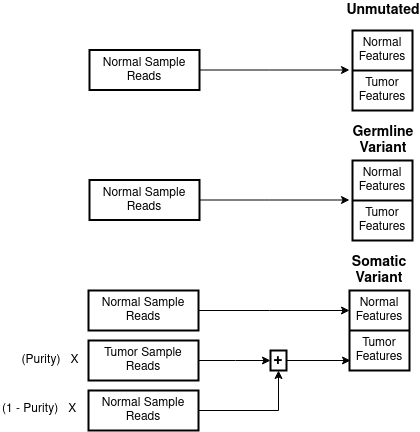
\includegraphics[width = 3in]{preprocess_initial}
\setlength{\belowcaptionskip}{0pt}
\caption{Initial data pre-processing from the normal and tumor sample reads into normal and tumor features. The purity parameter was set to 0.6.}
\label{preprocess_initial}
\vskip -5mm
\end{figure}

\subsection{Fixed and Modified Data Generation}

The initial data processing was not realistic and crucially, it only used the reads from the normal sample for both the ummutated and the germline variant locations, thereby making the tumor features simply copies of the normal features for those classes. The usage of the purity parameter was also incorrect, reads should not be combined based on it and it should be used for all classes, not just for somatic variants. 

As such, the data generation was modified after the first set of experiments were conducted to fix some of these issues and make the data model more realistic. Labelling the positions in the VCF file was done differently as well. Previously the germline variants were the mutations present in the normal sample and the somatic variants were the mutations in the tumor sample that are not present in the normal sample. In the modified version the mutations in the tumor sample that are present in the normal sample were considered as the germline mutations, and the rest of the tumor sample mutations were considered as the somatic variants. 

Note that the somatic variants were still the tumor sample mutations that are unique to the tumor sample, but the number of samples belonging to this class size did change. This could also be due to a chance in the official VCF file that occured between the two types of data generation. More details about the size and class distribution of the final dataset are shown in the next section.

In the new pre-processing normal and tumor sample reads for all locations were considered, while previously tumor sample reads were only fetched at locations labelled as somatic variants. This led to a slight increase in runtime: previously the pre-processing took around 1 hour, after the changes it took around 2 hours on the Eddie cluster.

For the unmutated and somatic variant locations 1-purity times the normal sample reads were used for the normal features and purity times the tumor sample reads were used the tumor features. For the germline variants the procedure was a bit special. For the tumor features, simply purity times the tumor sample reads were used, but for the normal features these same reads were taken and some small normal noise was applied to  it with mean 0 and variance 0.1, i.e.:$ \mathcal{N}(0,0.1)\, $.

Two additional features were added to the classification task data: fraction of gap reads for both normal and tumor sample (similarly to those use in the genotyping data), bring up the total number of features in this data to 6. Overall these changes made the signal in the data stronger as will be shown by the difference between the results in chapter 4. A demonstration can be seen on Figure 2.2.

\begin{figure}
\centering
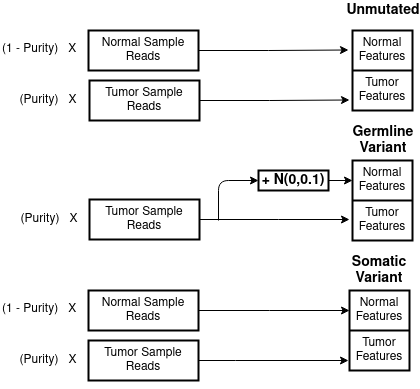
\includegraphics[width = 3in]{preprocess_tweaked}
\setlength{\belowcaptionskip}{0pt}
\caption{Tweaked data pre-processing from the normal and tumor sample reads into normal and tumor features. The purity parameter was set to 0.6.}
\label{preprocess_tweaked}
\vskip -5mm
\end{figure}

\section{Dataset Building}

After all locations in the genomic regions were processed, the data for the tumor and normal samples are saved in separate txt files. Altogether the number of locations was around 9.5 million for the training set and around 10 million for the test set.

The next step in the pipeline was building the dataset that the models consume from this intermediate representation. 

First all of the locations that were labelled as germline or somatic variants were extracted and a small window of the data was taken around these target locations, controlled by the context size parameter. All data was generated with a context size of 40, meaning 40 positions upstream and downstream from the target location, alongside the target location itself were collected into a single datapoint. At each position in this datapoint all the features used for the specific task the data was created for (classification or genotyping) were put taken from their respective samples and put as the rows of the data matrix.

In the data for the classification task this involved 4 features for the initial data and 6 for the modified one. As described previously these were normal reference nucleotide reads fraction (Normal Ref), normal alternate nucleotide reads fraction (Normal Alt), normal gap reads fraction (Normal Gap, omitted in initial data) and the same 3 for the tumor sample (with Tumor Gap omitted in the initial data). A visual representation of this can be seen in Figure 2.3.

In the data for the genotyping task there are 10 features, the fractions of reads corresponding to the 4 different types of nucleotides (Normal A, Normal T, Normal C, Normal G) and to the gap reads (Normal Gap) in the normal sample, and the same 5 features for the tumor sample. A demonstration is shown in Figure 2.4.

\begin{figure}
\centering
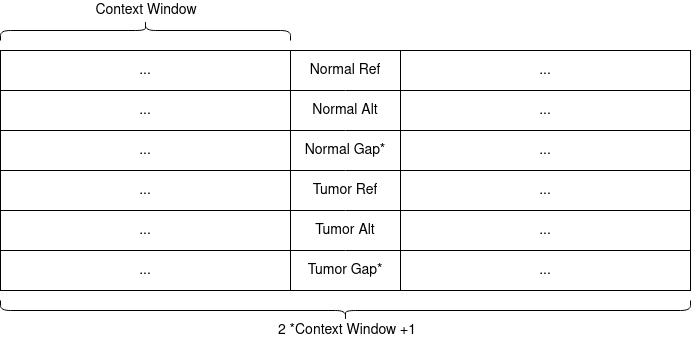
\includegraphics[width = 5in]{classification_features}
\setlength{\belowcaptionskip}{0pt}
\caption{Format of a data sample with its features of the classification task data. Features marked with * are only present in the modified data, not the initial. The context window used is 40 positions with each data point being 6x81 (4x81 in the initial data).}
\label{classification_features}
\vskip -5mm
\end{figure}

All of the positions that appeared in the targets and their context windows were recorded and an index set from the unused positions was created. The target locations corresponding to the unmutated, i.e. normal class were randomly drawn from these indices and then processed similarly. The number of unmutated locations chosen were the sum the germline variant and the somatic variant locations. The random seed used in the random state of the sampling has been set my student number as its seed for reproducibility.

As the final step, one-hot encoded labels of the classes were created in the form

\begin{center}
$ Germline Variant - [1,0,0] ~~~~ Somatic Variant - [0,1,0] ~~~~ Normal - [0,0,1] $
\end{center}

for the classification task and

\begin{center}
$ A - [1,0,0,0] ~~~~ T - [0,1,0,0] ~~~~ C - [0,0,1,0] ~~~~ G - [0,0,0,1] $
\end{center}

for the genotyping class. The data points and the labels of each class were concatenated and then shuffled using the same random state as for the sampling.

\begin{figure}
\centering
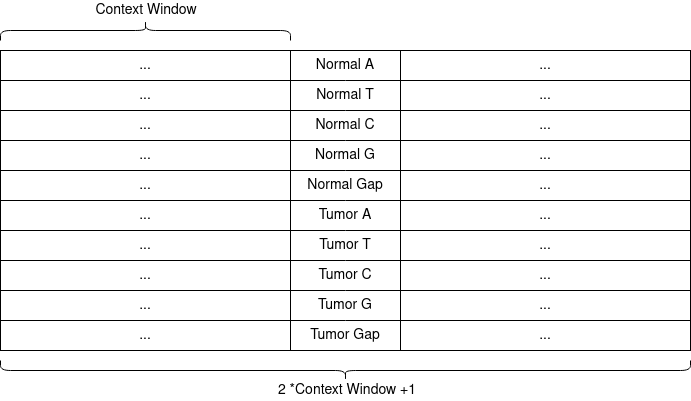
\includegraphics[width = 5in]{genotyping_features}
\setlength{\belowcaptionskip}{0pt}
\caption{Format of a data sample with its features of the genotyping task data. The context window used is 40 positions with each data point being 10x81.}
\label{classification_features}
\vskip -5mm
\end{figure}

Overall the number of classes and the total sizes of the processed datasets created were the following. Note that later 10\% of the training set was taken as a validation set, the size of which is also shown below.

Training and validation set, initial version:

\begin{itemize}

\item Germline variants: 5322 
\item Somatic variant: 1872 
\item Normal (unmutated): 7194 
\item Total training set size: 12950 
\item Total validation set size: 1438

\end{itemize}

Test set, initial version:

\begin{itemize}

\item Germline variants: 5264 
\item Somatic variant: 2269 
\item Normal (unmutated): 7533
\item Total test set size: 15066 

\end{itemize}

Training and validation set, modified version:

\begin{itemize}

\item Germline variants: 2464 
\item Somatic variant: 1859 
\item Normal (unmutated): 4323 
\item Total training set size: 7781 
\item Total validation set size: 865

\end{itemize}

Test set, modified version:

\begin{itemize}

\item Germline variants: 2809 
\item Somatic variant: 1691 
\item Normal (unmutated): 4500
\item Total test set size: 9000 

\end{itemize}

As noted in the previous section, the decrease in number of samples between the two version could be due to only taking the mutations from the tumor sample's VCF as both the germline and somatic variants, conditioned on whether they are present in the normal sample's VCF as well. However, this only explains the decrease in the number of germline variants. For somatic variants the change could be due to an update that occurred in the tumor sample's VCF (HG001, Utah woman standard reference genome) in the GIAB dataset. The number of normal (unmutated) datapoints is always just the sum of the previous two.

This chapter has explained the data, its format and the process of obtaining it. The next chapter focuses on  the introduction of the models used.




\chapter{Deep Neural Network Architectures}

This chapter introduces the neural network architectures that have been experimented with. These were the following: single layer Perceptron, vanilla RNN, LSTM, GRU and a very basic Transformer.

Fully connected feedforward neural networks are powerful and flexible models. In theory they are universal approximators that can fit any function given enough nodes in a single hidden layer with some nonlinearity applied to the outputs.

Even a simple, single layer perceptron can be used in many cases when the task is binary classification. Linear classifiers can work well diverse types of data even without having to apply nonlinearities.

Hence, although my tasks fall into the multiclass classification category, the first model tried to form a sort of baseline was such a single layer Perceptron, a single layer of fully connected nodes of the sequence of a data point mapped to the nodes representing the different classes.

A softmax layer is applied to the output, a nonlinear transformation that ensures that the final result is a probability distribution over the classes, easing comparison and interpretation of the model's best choice. It is defined as follows:

\begin{center}
$ \sigma (z_i) = exp(z_i) / \sum_{j=1}^K exp(z_j) $
\end{center}

Since the result is a probability distribution over the values, they will all fall in the [0,1] range and sum to 1. The output of all other models were fed through the same softmax activation function as well.

\section{Recurrent Neural Network Architectures}

A big drawback of such simple fully connected models is that they have no memory. Previously encountered inputs that could give useful context to correctly process present and future ones is not taken advantage of. 

This limitation is especially apparent in domains like natural language processing or really in any sequential or time series data analysis.

To remedy this issue, a special class of neural networks was created called recurrent neural networks (RNNs for short). RNNs have many varieties but the core idea around them is the same. A recurrent connection is introduced to create a loop with which the network can modify an internal state in light of the current data processed. This internal state encodes information about the previously seen data. 

This setup can also be thought of as several copies of the same network, each having an extra input and output. These networks pass on their internal state to the next network in line and accept the previous network's internal state as an input of their own.

As the length of the sequence to be processed increases a probem arises with vanilla RNN setups. Theoretically all information about earlier parts of the sequence should be well represented and easily taken into account when making inferences, learning connections between elements of the sequence. In practice this does not happen, as the gradient signal that drives the learning mechanism of backpropagation simply vanishes as a result of many multiplications with smaller and smaller values. The contribution of early elements to the loss of the later elements diminishes and long range dependencies are not learned.

To remedy this issue, several improved architectures have been developed. All of these have their own merits and may be useful on specific data. The most widespread variants are the Long Short Term Memory and the Gated Recurrent Unit architectures.

\section{Long Short Term Memory}

Long Short Term Memory networks or LSTMs are not a new addition to the zoo of neural networks. The architecture was first introduced in 1997 \cite{lstm} and soon proved to be very useful on a wide range of problems.

In the standard RNN architecture there is only one internal state and the hyperbolic tangent activation function applied to the output of it. In contrast an LSTM cell has four internal sub-components with 3 "gates". Figure 3.1 provides an overview of this structure.


\begin{figure}
\centering
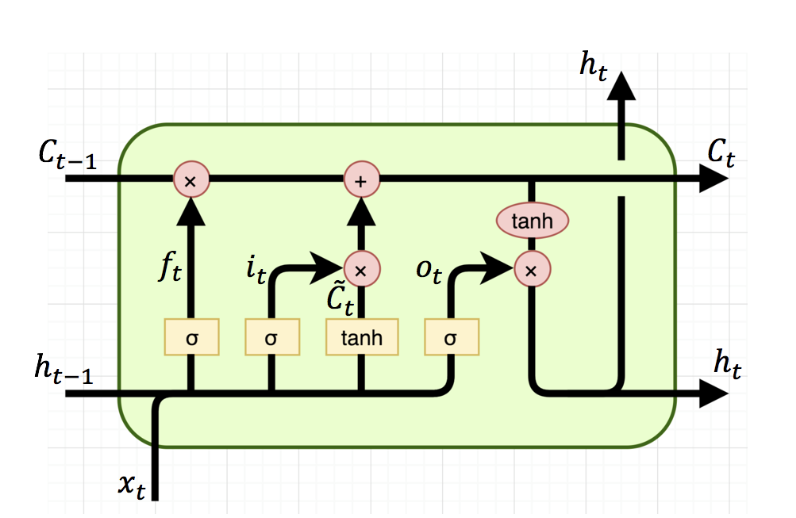
\includegraphics[width = 6in]{lstm}
\setlength{\belowcaptionskip}{0pt}
\caption{Illustration of the internal configurations of an LSTM cell. Image source: https://medium.com/@saurabh.rathor092/simple-rnn-vs-gru-vs-lstm-difference-lies-in-more-flexible-control-5f33e07b1e57}
\label{lstm}
\vskip -5mm
\end{figure}


There are 3 inputs to the LSTM cell, $ x_t $ the input data at time step t,  $ c_{t-1} $ the previous cell state and $ h_{t-1} $ the previous hidden state. The outputs are the current cell state and hidden state ( $ c_t, h_t $ ) with the hidden state serving as the model output as well.

The first operation that gets applied to the inputs is the forget gate, denoted by $ f_t $. Mathematically it is defined as:

\begin{center}
$ f_t = \sigma(W_f*[h_{t-1},x_t] + b_f) $
\end{center}

where $ \sigma $ denotes a standard sigmoid function and $ W_f, b_f $ are the weights and biases associated with the forget gate. The part with square brackets means the weights are applied to both the previous hidden state and the inputs, and then combined using a Hadamard (elementwise) product.

The name points to the functionality, the forget gate considers the previous hidden state and the incoming input two decide how much of the previous cell state should be forgotten. A value of 0 means complete wiping of the cell state, while 1 means no forgetting. This is applied to the cell state via a multiplication.

The next step is deciding how much of the input information should be saved in the new cell state. This is done via combining two operations, an input gate and a tanh layer that creates the candidate values. These are defined as:

\begin{center}
$ i_t = \sigma(W_i*[h_{t-1}, x_t] + b_i) $
\end{center}

\begin{center}
$ \tilde{C_t} = tanh(W_C*[h_{t-1},x_t] + b_C) $
\end{center}

Where all variables are defined similarly as before. The input gate decides how much of the new candidate values to memorise, while the tanh layer is applied to the previous hidden state and inputs to create these values. The two are combined via multiplication and then added to the cell state.

Then the update of the cell state can be written down as:

\begin{center}
$ C_t = f_t*C_{t-1}+i_t*\tilde{C_t} $
\end{center}

the output, that is the hidden state is based on this cell state. A tanh operation is applied to it to push the values between -1 and 1, and then multiplied with an output gate to produce the output of $ h_t $. This can be written as:

\begin{center}
$ o_t = \sigma(W_o*[h_{t-1},x_t] + b_o) $
\end{center}

\begin{center}
$ h_t = o_t*tanh(C_t) $
\end{center}

The parameters of these gates are also optimised during the learning process and in practice this makes the LSTM setup overcome the weaknesses of the vanilla RNN.

\section{Gated Recurrent Unit}

\begin{figure}
\centering
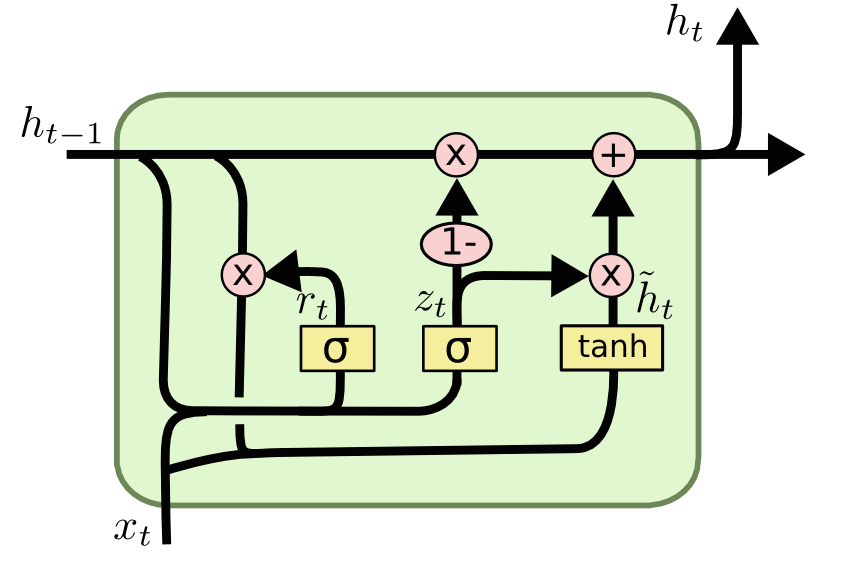
\includegraphics[width = 6in]{gru}
\setlength{\belowcaptionskip}{0pt}
\caption{Illustration of the internal configurations of a GRU cell. Image source: https://medium.com/@saurabh.rathor092/simple-rnn-vs-gru-vs-lstm-difference-lies-in-more-flexible-control-5f33e07b1e57}
\label{gru}
\vskip -5mm
\end{figure}

Gated Recurrent Unit or GRU, is a more recent architecture from 2014, presented in \cite{gru}. It is essentially a simplification of the LSTM cell albeit it may not seem that way upon first inspection. An illustration of the GRU cell is presented in Figure 3.2.

The main changes compared to LSTM are the combination of input and forget gates into an update gate and the merging of the cell and hidden states.

The update gate decides how much of the previously stored hidden state is passed along. The equation is simlar to the ones before, but there is no bias involved:

\begin{center}
$ z_t = \sigma(W_z*[h_{t-1},x_t]) $
\end{center}

$ r_t $ stands for the reset gate of the current timestep, which is defined very similarly to the update gate:

\begin{center}
$ r_t = \sigma(W_r*[h_{t-1}, x_t]) $
\end{center}

This gate decides what information should be removed from the total that has been accumulated in the previous hidden state.

Next the reset gate and the inputs are used to determine what parts of the previous hidden state should be propagated in the following way:

\begin{center}
$ \tilde{h_t} = tanh(W*[r_t*h_{t-1}, x_t]) $
\end{center}

Finally this is added to the hidden state after the 1 minus the results of the update gate is multiplied by the previous value:

\begin{center}
$ h_t = (1-z_t)*h_{t-1} + z_t*\tilde{h_t} $
\end{center}

This architecture has also successfully combatted the vanishing gradient problem and is in widespread use due to its great performance.

\section{Transformer}

The Transformer is a novel architecture type from 2017, introduced in \cite{transformer}. Since the original paper being somewhat impenetrable, a simpler and clearer introduction is given a famous blogpost \cite{transformer-blog}, on which the explanation here is based on.

The fundamental building block of this architecture is the self-attention operation. Initially people started to use this operation to augment RNNs, especially in sequence-to-sequence tasks where encoder-decoder architectures are used. In these architectures there are two models (usually some RNNs, for instance LSTMs), an encoder which transforms the input sequence into a more compact intermediate representation and a decoder which takes this representation and sequentially builds an output sequence from it.

Self-attention in this context is most often used in the decoder part. The operation is simply a weighted average of an input: 

\begin{center}
$ y_i = \sum_j w_{ij} * x_j $
\end{center}

Where the weights are obtained from the data, more specifically usually produced via a dot product:

\begin{center}
$ w_{ij} = x_i^T x_j $ 
\end{center}

These weights are scaled via the a softmax before used for calculating $ y_i $ , which was shown before. When used in a decoder model, the attention weights are used to put emphasis on the more important parts of the sequence rather instead of assuming that all parts are equally important.

Using self-attention improved performance and in some cases was adapted in the encoder as well to assign weights to the inputs as well. Naturally, the question arose if this mechanism could work in itself without requiring the original recurrent models.

Surprisingly the answer was yes, which lead to the Transformer architecture and it's great success. However, there is more to this model than the simple self-attention mechanism. 

First of all, three different roles are filled by each input. These are query, key and value. An input is a query when it is compared to all other inputs to produce weight for its own output, it is a key when it is compared to other inputs to produce their output weights, and finally it is a value when it is used in the finally weighted sum to produce the output. Described with equations:

\begin{center}
$ q_i = W_q x_i ~~~~~~~~ k_i = W_k x_i ~~~~~~~~ v_i = W_v x_i $

$ w_{ij}^\prime = q_i^T k_j $

$ w_{ij} = softmax(w_{ij}^\prime)$

$ y_i = \sum_{j} w_{ij} v_j $
\end{center}

Notice that three weight matrices were added to differentiate the inputs for their different usages. These are just linear transformations, but they add parameters that can be tuned during model training. An illustration of this is shown in Figure 3.3. 

\begin{figure}
\centering
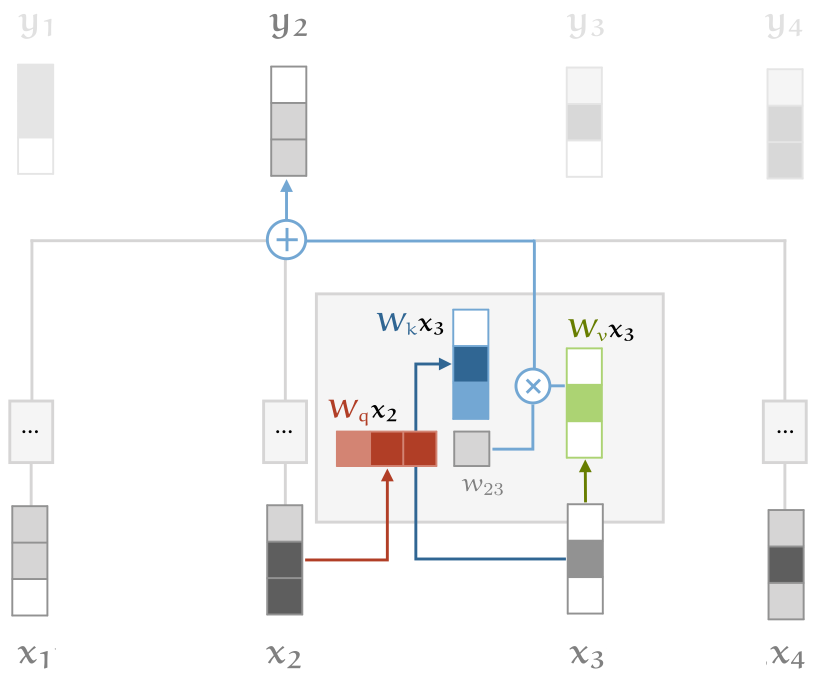
\includegraphics[width = 5in]{key-query-value}
\setlength{\belowcaptionskip}{0pt}
\caption{Self-attention mechanism with key, query and value linear transformations (softmax not indicated). Image source: http://peterbloem.nl/blog/transformers}
\label{gru}
\vskip -5mm
\end{figure}

Usually the unnormalised weights $ w_{ij}^\prime $ are scaled by a factor of the square root of the input vector dimension to avoid saturation and with it impediment to the learning in the softmax function, which is sensitive to very large values.

The last addition to the attention mechanism that needs to be considered is a splitting into multiple heads. This just means that instead of a single focus, there can be multiple ones. Multiple $ W_q, W_k, W_v $ matrices are defined which combined with the same input can lead to different values. These are then concatenated and put through a linear transformation to get back to the original dimensionality.

This setup is called wide self-attention. A computationally cheaper and more memory efficient alternative is splitting up the input into as many parts as there are attention heads and letting each head attend only to its designated chunk of the input.

A Transformer block, in addition to self-attention, also contains a layer normalisation after the attention, a fully connected feedforward layer applied to each input individually, followed by another layer normalisation. Residual connections are used as well to connect the inputs to the the self-attention and feedforward layers to their outputs before normalisation. Layer normalisation usually just means scaling and shifting the values to have a mean of zero and unit variance. A complete Transformer block is illustrated in Figure 3.4. 

\begin{figure}
\centering
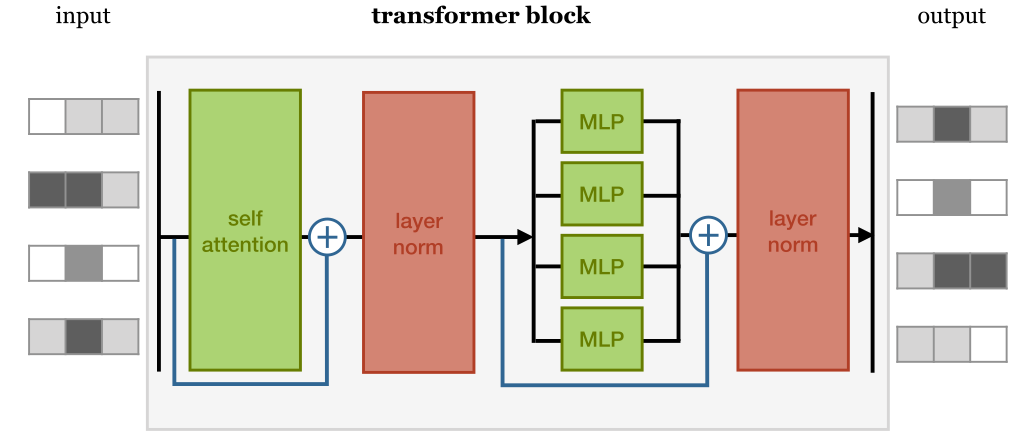
\includegraphics[width = 5in]{transformer-block}
\setlength{\belowcaptionskip}{0pt}
\caption{A full Transformer block. MLP (multi-layer perceptron) refers to a single fully connected feedforward layer. The plus signs indicate residual connections. Image source: http://peterbloem.nl/blog/transformers}
\label{gru}
\vskip -5mm
\end{figure}

Additionally since the sequential processing aspect of RNNs is lost in this setup, in many cases positional embeddings are added to the inputs to introduce a notion of positions in the sequence for Transformers as well.

Transformers work remarkably well and in the past few years have been gradually replacing RNNs in many contexts, and recently even CNNs in some Computer Vision tasks (e.g. Vision Transformer \cite{vision-transformer}). 

Due to the basic Transformer block having relatively few parameters and high efficiency compared to for instance LSTM layers, there has been a tendency to scale up Transformer models to previously unseen sizes, resulting in enormous number of parameters and breakthrough performance. Some famous examples are Google's BERT \cite{bert} and OpenAI's GPT-3 \cite{gpt-3}.

The model used in this work is was simple in comparison. The setup of it and the other previously mentioned models is introduced in the next chapter.




\chapter{Experiments and Results}

This final chapter describes all of the experiments conducted, their results and what can be concluded from them. The first section deals with the classification task, related experiments and the model setups. The second section introduces the other main task, genotyping, and the results for it.

All of the code used for the project can be found in a GitHub repository\footnote{\url{https://github.com/self-improving-agent/somatic-variant-calling-with-deep-learning}}, which also contains a Sphinx documentation. Some of the scripts have two versions, with one of them containing the LOCAL suffix. Both have the same functionality but the suffixed ones are designed to be run from the command line as python scripts, while the ones without it are the main scripts that can be used via Snakemake rules and auxiliary bash scripts, and run on a cluster. 

\section{Setup}

Last year's project has served as the starting point for defining my models. The types of models defined in it were: vanilla RNN, LSTM, GRU, Perceptron. All of these were reused and a simple Transformer was added. The architecture setup for these is the following.

For the RNN based models first the input is fed into the specific type of recurrent block used (RNN, LSTM or GRU), where the hyperparameter choices are the number of layers, the number of hidden units in the layers, the amount of dropout to be applied after each layer (reference to dropout \cite{dropout}), and whether the recurrent block should be bidirectional. 

If the recurrent block is bidirectional, the output of it is taken from both sides and concatenated. If some positive amount of dropout is defined, an additional dropout layer is applied to the output. Then a fully connected linear layer is applied mapping from the number of hidden units used to the number of classes (three for classification, four for genotyping). Finally, a softmax layer is applied to normalise these outputs.

For the Perceptron model, there is only one fully connected linear layer mapping a flattened vector of length of input sequence times the number of features (81*4 or 81*6 for classification, 81*10 for genotyping) to the number of classes. A softmax layer is applied to the resulting output.

The Transformer model is the most complicated and computationally expensive of the models tried, although it is still much simpler than the large scale architectures used commercially. Since this is not a sequence-to-sequence application, only encoding is needed to create a representation of the input, decoding from this representation can be omitted and the replaced with the linear layer and softmax used for the other models.

A Transformer encoder layer is defined with as many attention heads as number of features, optionally with some amount of dropout. This layer is the Pytorch implementation of a full Transformer block (for the description of it see section 3.4). The number of encoder layers to be used is a hyperparameter choice.

The outputs of this layer is are flattened (after a possible dropout layer) and a linear layer is applied of similar dimensions of that of the Perceptron model: sequence length times number of features to number of classes. After a final softmax layer, the output is completed.

These types of models were considered with their associated hypterparameters as well two universal ones: the batch size and the learning rate. For all models the Adam optimiser is used \cite{adam} to tune model parameters and the loss is measured via cross entropy, as is standard in multiclass classification approaches.

At each batch, at the end of each training epoch and when testing a model, a confusion matrix is built from the model predictions to extract the true and false positives and negatives and calculate the evaluation metrics from them. 

The metrics tracked throughout the experiments are the following standard metrics:

\begin{center}
$ Accuracy = {True~Positives + True~Negatives \over True~Positives + True~Negatives + False~Positives + False~Negatives}   $

$ Precision = {True~Positives \over True~Positives + False~Positives}   $

$ Recall = {True~Positives \over True~Positives + False~Negatives}   $

$ F1~Score = {2*Precision*Recall \over Precision + Recall}   $
\end{center}

Additionally for the validation and test sets the area under curve (AUC) statistic of the Receiver Operating Characteristic (ROC) curve is recorded as well. The ROC curve measures the true positive rate against the false positive rate and gives a good picture of a model's performance at different levels of false positive rate. A perfect classifier has an AUC of 1.0.

During both training and testing the metrics in all of the runs are recorded and graphs are produced to show how they evolve over time. All of the examples that will be shown in this chapter are taken from these, however a lot of them have to be omitted for brevity. They can be found in the repository that accompanies this work. Model checkpoints are saved as well for producing graphs for the test set performance over time, as well as for allowing for the training to be stopped and continued at any time.

Note that not all experiments in the result folders may contain all of the things described here, or the same graphs, etc. Functionality was implemented incrementally and improved bit by bit, in this text the emphasis is on the final version and its features. The experiments in the main results folder are the last and most complete ones, but the older ones are recorded as well for completeness, they can be found in the old\_results and the even\_older\_results folders. All folders named "Test" are functionality tests not actual experiments.

\section{Classification Task}

In the classification task the goal is to tell whether the target location is a germline variant, a somatic variant or a normal, unmutated base. The input to all models are formatted data matrices described in chapter 2, with 4 and then eventually 6 rows and 81 columns (40 positions upstream and downstream from the target location, along with the target location itself), and the output is one of the three classes.

\subsection{Initial Experiments}

Short training runs of 100 epochs over the training data were run to determine the best hyperparameters for the models. For the recurrent models the hyperparameters found in my project last year were taken as the starting point.

The best performing hyperparameters ended up being:

\begin{itemize}

\item Batch Size: 250 
\item Learning Rate: 0.001 
\item Reccurent Models Hidden Units : 32
\item Recurrent Models Hidden Layers: 2
\item Transformer Encoder Layers: 1 (2 with relatively few training epochs)

\end{itemize}

Using dropout and bidirectionality were evaluated throughout all stages of experimentation with the former being either 5\% or 10\% and the latter either being used or not used. More dropout was not used since the the preliminary hyperparameter search showed that higher values started to significantly worsen results.

After the best hyperparameters have been determined, the initial experiments were conducted with a training duration of 1000 epochs. Each models were trained 10 times and the results were averaged over the runs for the final results and plotting. The only exception is the Transformer model which was only trained 4 times at this stage since it was discovered that using 1 encoder layers instead of 2 could work better over more training epochs.

Tables 4.1-4.3 present the results of all of the models on the training, validation and test sets. Table 4.4 shows the performances on the AUC metric separately for the validation and test sets. All results are reported with standard error, also averaged over the 10 runs.

On the training and validation sets the simple Perceptron model dominates all metrics by a significant margin. It also beats the other models in terms of validation and and test set AUC. On the test set things look a bit more varied as the bidirectional GRU model with 5\% added dropout is narrowly beating the Perceptron.

The reason for only training GRU models with bidirectionality and dropout is simply due to the fact that out of the simple recurrent models the GRU has performed the best. In the small scale hyperparameter experimentation the other models were also tried with bidirectionality and dropout, but they all seemed to have been under-performing compared to the GRU, so they were discarded to decrease the number of models that had to be trained.

\begin{table}
%\vskip -7mm
\begin{center}
\caption{Training set performance of all model types in the first experiment, averaged over 10 runs. The Transformer model was only run 4 times and with 2 encoder layers}
\resizebox{12cm}{!}{
\begin{tabular}{ |p{6cm}||p{2.5cm}|p{2.5cm}|p{2.5cm}|p{2.5cm}| }
 \hline
 \multicolumn{5}{|c|}{1000 Epochs, Training Set Results} \\
 \hline
 \textbf{Model} & \textbf{Accuracy} & \textbf{Precision} & \textbf{Recall} &  \textbf{F1 Score}\\
 \hline
 GRU  & \small{95.35$ \%~\pm $ 0.74}   & \small{95.27$ \%~\pm $ 0.56} & \small{89.52$ \%~\pm $ 2.82} & \small{92.12$ \%~\pm $ 1.91} \\ 
 \hline
 LSTM & \small{84.7$ \%~\pm $ 3.7} & \small{61.7$ \%~\pm $ 9.25} & \small{64.73$ \%~\pm $ 7.28} & \small{62.57$ \%~\pm $ 8.48} \\
 \hline
 Vanilla RNN & \small{71.49$ \%~\pm $ 2.3} & \small{57.23$ \%~\pm $ 6.96} & \small{40.89$ \%~\pm $ 2.55} & \small{45.9$ \%~\pm $ 3.79} \\
 \hline
 Perceptron & \textbf{\small{96.86$ \%~\pm $ 0.0}} & \textbf{\small{97.03$ \%~\pm $ 0.0}} & \textbf{\small{93.78$ \%~\pm $ 0.01}} & \textbf{\small{95.38$ \%~\pm $ 0.0}} \\
 \hline
 GRU + 5\% Dropout & \small{96.33$ \%~\pm $ 0.04} & \small{96.08$ \%~\pm $ 0.1} & \small{92.76$ \%~\pm $ 0.05} & \small{94.39$ \%~\pm $ 0.07} \\
 \hline
 GRU + 10\% Dropout & \small{95.47$ \%~\pm $ 0.76} & \small{91.85$ \%~\pm $ 3.9} & \small{89.72$ \%~\pm $ 2.85} & \small{90.74$ \%~\pm $ 3.4} \\
 \hline
 Bidirectional GRU & \small{85.55$ \%~\pm $ 4.86} & \small{79.17$ \%~\pm $ 10.58} & \small{80.74$ \%~\pm $ 7.5} & \small{78.95$ \%~\pm $ 9.66} \\
 \hline
 Bidirectional GRU + 5\% Dropout & \small{96.44$ \%~\pm $ 0.04} & \small{96.32$ \%~\pm $ 0.07} & \small{92.96$ \%~\pm $ 0.1} & \small{94.61$ \%~\pm $ 0.07} \\
 \hline
 Bidirectional GRU + 10\% Dropout & \small{96.3$ \%~\pm $ 0.08} & \small{96.03$ \%~\pm $ 0.17} & \small{92.81$ \%~\pm $ 0.15} & \small{94.39$ \%~\pm $ 0.15} \\
 \hline
 Transformer$^* $ & \small{96.21$ \%~\pm $ 0.07} & \small{96.32$ \%~\pm $ 0.11} & \small{92.61$ \%~\pm $ 0.11} & \small{94.42$ \%~\pm $ 0.1} \\
 \hline

\end{tabular}
}
\vskip -5mm
\end{center}
\end{table}

\begin{table}
%\vskip -20mm
\begin{center}
\caption{Validation set performance of all model types in the first experiment, averaged over 10 runs. The Transformer model was only run 4 times and with 2 encoder layers}
\resizebox{12cm}{!}{
\begin{tabular}{ |p{6cm}||p{2.5cm}|p{2.5cm}|p{2.5cm}|p{2.5cm}| }
 \hline
 \multicolumn{5}{|c|}{1000 Epochs, Validation Set Results} \\
 \hline
 \textbf{Model} & \textbf{Accuracy} & \textbf{Precision} & \textbf{Recall} &  \textbf{F1 Score}\\
 \hline
 GRU  & \small{94.51$ \%~\pm $ 0.79} & \small{90.95$ \%~\pm $ 3.79} & \small{89.14$ \%~\pm $ 2.88} & \small{90.01$ \%~\pm $ 3.35} \\ 
 \hline
 LSTM & \small{83.59$ \%~\pm $ 3.93} & \small{61.0$ \%~\pm $ 9.37} & \small{65.14$ \%~\pm $ 7.5} & \small{62.34$ \%~\pm $ 8.69} \\
 \hline
 Vanilla RNN & \small{70.43$ \%~\pm $ 2.21} & \small{45.38$ \%~\pm $ 3.99} & \small{41.28$ \%~\pm $ 2.53} & \small{42.4$ \%~\pm $ 3.17} \\
 \hline
 Perceptron & \textbf{\small{96.24$ \%~\pm $ 0.01}} & \textbf{\small{96.3$ \%~\pm $ 0.01}} & \textbf{\small{93.72$ \%~\pm $ 0.03}} & \textbf{\small{94.99$ \%~\pm $ 0.02}} \\
 \hline
 GRU + 5\% Dropout & \small{95.48$ \%~\pm $ 0.06} & \small{95.06$ \%~\pm $ 0.09} & \small{92.36$ \%~\pm $ 0.09} & \small{93.69$ \%~\pm $ 0.08} \\
 \hline
 GRU + 10\% Dropout & \small{94.59$ \%~\pm $ 0.82} & \small{90.88$ \%~\pm $ 3.92} & \small{89.23$ \%~\pm $ 2.91} & \small{90.01$ \%~\pm $ 3.44} \\
 \hline
 Bidirectional GRU & \small{88.32$ \%~\pm $ 4.55} & \small{78.66$ \%~\pm $ 10.36} & \small{80.6$ \%~\pm $ 7.47} & \small{78.73$ \%~\pm $ 9.47} \\
 \hline
 Bidirectional GRU + 5\% Dropout & \small{95.62$ \%~\pm $ 0.06} & \small{95.26$ \%~\pm $ 0.07} & \small{92.56$ \%~\pm $ 0.1} & \small{93.89$ \%~\pm $ 0.07} \\
 \hline
 Bidirectional GRU + 10\% Dropout & \small{95.46$ \%~\pm $ 0.09} & \small{95.03$ \%~\pm $ 0.14} & \small{92.32$ \%~\pm $ 0.2} & \small{93.65$ \%~\pm $ 0.16} \\
 \hline
 Transformer$^* $ & \small{90.74$ \%~\pm $ 0.07} & \small{89.41$ \%~\pm $ 0.05} & \small{85.09$ \%~\pm $ 0.14} & \small{87.2$ \%~\pm $ 0.09} \\
 \hline

\end{tabular}
}
\vskip -5mm
\end{center}
\end{table}

\begin{table}
%\vskip -14mm
\begin{center}
\caption{Test set performance of all model types in the first experiment, averaged over 10 runs. The Transformer model was only run 4 times and with 2 encoder layers}
\resizebox{12cm}{!}{
\begin{tabular}{ |p{6cm}||p{2.5cm}|p{2.5cm}|p{2.5cm}|p{2.5cm}| }
 \hline
 \multicolumn{5}{|c|}{1000 Epochs, Test Set Results} \\
 \hline
 \textbf{Model} & \textbf{Accuracy} & \textbf{Precision} & \textbf{Recall} &  \textbf{F1 Score}\\
 \hline
 GRU  & \small{93.16$ \%~\pm $ 0.78} & \small{89.88$ \%~\pm $ 3.33} & \small{85.7$ \%~\pm $ 2.61} & \small{87.73$ \%~\pm $ 2.96} \\ 
 \hline
 LSTM & \small{83.11$ \%~\pm $ 3.51} & \small{60.03$ \%~\pm $ 9.18} & \small{63.17$ \%~\pm $ 6.96} & \small{60.95$ \%~\pm $ 8.28} \\
 \hline
 Vanilla RNN & \small{70.55$ \%~\pm $ 2.17} & \small{42.1$ \%~\pm $ 4.44} & \small{40.51$ \%~\pm $ 2.37} & \small{40.52$ \%~\pm $ 3.46} \\
 \hline
 Perceptron & \small{94.15$ \%~\pm $ 0.01} & \textbf{\small{94.15$ \%~\pm $ 0.01}} & \small{88.41$ \%~\pm $ 0.01} & \small{91.19$ \%~\pm $ 0.01} \\
 \hline
 GRU + 5\% Dropout & \small{94.06$ \%~\pm $ 0.03} & \small{93.48$ \%~\pm $ 0.12} & \small{88.51$ \%~\pm $ 0.08} & \small{90.93$ \%~\pm $ 0.08} \\
 \hline
 GRU + 10\% Dropout & \small{93.18$ \%~\pm $ 0.77} & \small{89.35$ \%~\pm $ 3.81} & \small{85.35$ \%~\pm $ 3.81} & \small{87.45$ \%~\pm $ 3.22} \\
 \hline
 Bidirectional GRU & \small{86.58$ \%~\pm $ 4.74} & \small{77.12$ \%~\pm $ 10.35} & \small{77.5$ \%~\pm $ 6.98} & \small{76.21$ \%~\pm $ 9.32} \\
 \hline
 Bidirectional GRU + 5\% Dropout & \textbf{\small{94.18$ \%~\pm $ 0.03}} & \small{93.91$ \%~\pm $ 0.05} & \textbf{\small{88.67$ \%~\pm $ 0.1}} & \textbf{\small{91.21$ \%~\pm $ 0.07}} \\
 \hline
 Bidirectional GRU + 10\% Dropout & \small{94.11$ \%~\pm $ 0.04} & \small{93.67$ \%~\pm $ 0.07} & \small{88.56$ \%~\pm $ 0.12} & \small{91.04$ \%~\pm $ 0.09} \\
 \hline
 Transformer$^* $ & \small{79.93$ \%~\pm $ 10.02} & \small{70.44$ \%~\pm $ 12.51} & \small{67.33$ \%~\pm $ 11.96} & \small{68.78$ \%~\pm $ 12.22} \\
 \hline

\end{tabular}
}
\vskip -5mm
\end{center}
\end{table}

\begin{table}
\begin{center}
\caption{AUC metric performance of all model types in the first experiment, averaged over 10 runs. The Transformer model was only run 4 times and with 2 encoder layers}
\resizebox{12cm}{!}{
\begin{tabular}{ |p{6cm}||p{3cm}|p{3cm}| }
 \hline
 \multicolumn{3}{|c|}{1000 Epochs, AUCs} \\
 \hline
 \textbf{Model} & \textbf{Validation AUC} & \textbf{Test AUC} \\
 \hline
 GRU  & \small{0.9213$ ~\pm $ 0.03} &  \small{0.902$ ~\pm $ 0.02} \\ 
 \hline
 LSTM & \small{0.8195$ ~\pm $ 0.05} & \small{0.7949$ ~\pm $ 0.05} \\
 \hline
 Vanilla RNN & \small{0.5373$ ~\pm $ 0.05} & \small{0.5447$ ~\pm $ 0.05} \\
 \hline
 Perceptron & \textbf{\small{0.9624$ ~\pm $ 0.0}} & \textbf{\small{0.9624$ ~\pm $ 0.0}} \\
 \hline
 GRU + 5\% Dropout & \small{0.9465$ ~\pm $ 0.0} & \small{0.9235$ ~\pm $ 0.0} \\
 \hline
 GRU + 10\% Dropout & \small{0.9457$ ~\pm $ 0.0} & \small{0.9232$ ~\pm $ 0.0} \\
 \hline
 Bidirectional GRU & \small{0.8444$ ~\pm $ 0.07} & \small{0.8272$ ~\pm $ 0.07} \\
 \hline
 Bidirectional GRU + 5\% Dropout & \small{0.9441$ ~\pm $ 0.0} & \small{0.9224$ ~\pm $ 0.0} \\
 \hline
 Bidirectional GRU + 10\% Dropout & \small{0.9478$ ~\pm $ 0.0} & \small{0.9252$ ~\pm $ 0.0} \\
 \hline
 Transformer$^* $ & \small{0.839$ ~\pm $ 0.0} & \small{0.7052$ ~\pm $ 0.14} \\
 \hline

\end{tabular}
}
\end{center}
\vskip -3mm
\end{table}

\subsection{Increased Training Time}

After the results of the previous sections were observed, it could be concluded that extending the training to 2000 epochs would be beneficial and could improve results. 

At this point another improvement was made. So far only the averages across classes were recorded for each metric, but from now on all metrics were recorded for all three classes to get more fine-grained data on performance. The tables here only report the averages that were manually calculated from the performances of the separate classes, but all graphs shown will have the class separation to draw more insights from.

In the training and validation sets the Perceptron was the best on all metrics of all classes, more variety was only present in the test set results where on most metrics the Perceptron had a better performance on the germline variant class while on the others the bidirectional GRU with 5\% dropout tended to outperform it. As such, showing the averaged results for the final performance does not result in a big loss in terms of the observed variability.

Tables 4.5-4.8 showcase results similarly to Table 4.1-4.4 of the previous section. A major difference is that these longer experiments were only run for the models that performed the best in the previous, shorter ones. This selection still showcases the variety in the types of models. The Transformer model used is the better performing 1 encoder layer version.

Overall the results improved for all of the models but the Peceptron still is a cut above the rest for the training and validation sets, while for the test set the bidirectional GRU with 5\% dropout still performs the best on all metrics except precision. Note that the error bars for the AUCs have been extended to four positions after the decimal point for a more accurate view into their behaviour.

\begin{table}
%\vskip -5mm
\begin{center}
\caption{Training set performance when training time was doubled.}
\resizebox{12cm}{!}{
\begin{tabular}{ |p{6cm}||p{2.5cm}|p{2.5cm}|p{2.5cm}|p{2.5cm}| }
 \hline
 \multicolumn{5}{|c|}{2000 Epochs, Training Set Results} \\
 \hline
 \textbf{Model} & \textbf{Accuracy} & \textbf{Precision} & \textbf{Recall} &  \textbf{F1 Score}\\
 \hline
 GRU  & \small{96.39$ \%~\pm $ 0.07} & \small{96.28$ \%~\pm $ 0.12} & \small{92.95$ \%~\pm $ 0.13} & \small{94.59$ \%~\pm $ 0.12} \\ 
 \hline
 Perceptron & \textbf{\small{96.85$ \%~\pm $ 0.01}} & \textbf{\small{97.1$ \%~\pm $ 0.01}} & \textbf{\small{94.01$ \%~\pm $ 0.01}} & \textbf{\small{95.53$ \%~\pm $ 0.01}} \\
 \hline
 Bidirectional GRU + 5\% Dropout & \small{96.74$ \%~\pm $ 0.03} & \small{96.67$ \%~\pm $ 0.09} & \small{93.63$ \%~\pm $ 0.11} & \small{95.13$ \%~\pm $ 0.07} \\
 \hline
 Transformer$ $ & \small{96.38$ \%~\pm $ 0.03} & \small{96.55$ \%~\pm $ 0.05} & \small{93.03$ \%~\pm $ 0.08} & \small{94.76$ \%~\pm $ 0.06} \\
 \hline

\end{tabular}
}
\end{center}
\vskip -3mm
\end{table}

\begin{table}
\begin{center}
\caption{Validation set performance when training time was doubled.}
\resizebox{12cm}{!}{
\begin{tabular}{ |p{6cm}||p{2.5cm}|p{2.5cm}|p{2.5cm}|p{2.5cm}| }
 \hline
 \multicolumn{5}{|c|}{2000 Epochs, Validation Set Results} \\
 \hline
 \textbf{Model} & \textbf{Accuracy} & \textbf{Precision} & \textbf{Recall} &  \textbf{F1 Score}\\
 \hline
 GRU  & \small{95.62$ \%~\pm $ 0.12} & \small{95.35$ \%~\pm $ 0.18} & \small{92.59$ \%~\pm $ 0.21} & \small{93.95$ \%~\pm $ 0.18} \\ 
 \hline
 Perceptron & \textbf{\small{96.46$ \%~\pm $ 0.02}} & \textbf{\small{96.5$ \%~\pm $ 0.03}} & \textbf{\small{94.18$ \%~\pm $ 0.03}} & \textbf{\small{95.32$ \%~\pm $ 0.02}} \\
 \hline
 Bidirectional GRU + 5\% Dropout & \small{95.97$ \%~\pm $ 0.05} & \small{95.67$ \%~\pm $ 0.12} & \small{93.34$ \%~\pm $ 0.14} & \small{94.49$ \%~\pm $ 0.09} \\
 \hline
 Transformer$ $ & \small{90.75$ \%~\pm $ 0.09} & \small{89.39$ \%~\pm $ 0.16} & \small{85.21$ \%~\pm $ 0.21} & \small{87.25$ \%~\pm $ 0.14} \\
 \hline

\end{tabular}
}
\end{center}
\vskip -5mm
\end{table}

\begin{table}
\begin{center}
\caption{Test set performance when training time was doubled.}
\resizebox{12cm}{!}{
\begin{tabular}{ |p{6cm}||p{2.5cm}|p{2.5cm}|p{2.5cm}|p{2.5cm}| }
 \hline
 \multicolumn{5}{|c|}{2000 Epochs, Test Set Results} \\
 \hline
 \textbf{Model} & \textbf{Accuracy} & \textbf{Precision} & \textbf{Recall} &  \textbf{F1 Score}\\
 \hline
 GRU  & \small{94.2$ \%~\pm $ 0.05} & \small{93.76$ \%~\pm $ 0.11} & \small{88.9$ \%~\pm $ 0.15} & \small{91.27$ \%~\pm $ 0.12} \\ 
 \hline
 Perceptron & \small{94.12$ \%~\pm $ 0.01} & \textbf{\small{94.1$ \%~\pm $ 0.03}} & \small{88.36$ \%~\pm $ 0.03} & \small{91.14$ \%~\pm $ 0.02} \\
 \hline
 Bidirectional GRU + 5\% Dropout & \textbf{\small{94.31$ \%~\pm $ 0.04}} & \small{93.97$ \%~\pm $ 0.1} & \textbf{\small{89.13$ \%~\pm $ 0.04}} & \textbf{\small{91.49$ \%~\pm $ 0.09}} \\
 \hline
 Transformer$ $ & \small{83.53$ \%~\pm $ 6.19} & \small{77.24$ \%~\pm $ 9.51} & \small{75.78$ \%~\pm $ 7.21} & \small{76.5$ \%~\pm $ 8.47} \\
 \hline

\end{tabular}
}
\end{center}
\vskip -5mm
\end{table}

\begin{table}
\begin{center}
\caption{AUC metric performance when training time was doubled.}
\resizebox{12cm}{!}{
\begin{tabular}{ |p{6cm}||p{3cm}|p{3cm}| }
 \hline
 \multicolumn{3}{|c|}{2000 Epochs, AUCs} \\
 \hline
 \textbf{Model} & \textbf{Validation AUC} & \textbf{Test AUC} \\
 \hline
 GRU  & \small{0.9485$ ~\pm $ 0.0035} & \small{0.9268$ ~\pm $ 0.0032} \\ 
 \hline
 Perceptron & \textbf{\small{0.9613$ ~\pm $ 0.0006}} & \textbf{\small{0.9281$ ~\pm $ 0.0007}} \\
 \hline
 Bidirectional GRU + 5\% Dropout & \small{0.952$ ~\pm $ 0.0019} & \small{0.9259$ ~\pm $ 0.0031} \\
 \hline
 Transformer$ $ & \small{0.8384$ ~\pm $ 0.0018} & \small{0.8382$ ~\pm $ 0.0514} \\
 \hline

\end{tabular}
}
\end{center}
\vskip -3mm
\end{table}

% Data tweak

It was at this point the the inadequacy of the data format was noticed and all of the data was re-designed and re-generated to improve the representation and make it more correct and a bit more realistic. For more details see section 2.2.2 and chapter 2 in general for the bigger picture about the data.

Since the data has changed, all models were trained from scratch again to see how the results changed for each. The new results are shown in Tables 4.9-4.12.

With this modified data the performance has increased significantly for the best performing models, while the simple recurrent models tended to do worse than before. The Perceptron still performs the best for both training and validation sets, but for the test set a new front-runner has emerged as the Transformer surpassed the performance of the previously best bidirectional GRU with 5\% dropout.


\begin{table}
\begin{center}
\caption{Training set performance on the modified data}
\resizebox{12cm}{!}{
\begin{tabular}{ |p{6cm}||p{2.5cm}|p{2.5cm}|p{2.5cm}|p{2.5cm}| }
 \hline
 \multicolumn{5}{|c|}{Modified Data, 2000 Epochs, Training Set Results} \\
 \hline
 \textbf{Model} & \textbf{Accuracy} & \textbf{Precision} & \textbf{Recall} &  \textbf{F1 Score}\\
 \hline
 GRU  & \small{89.6$ \%~\pm $ 5.3} & \small{81.65$ \%~\pm $ 9.9} & \small{81.93$ \%~\pm $ 10.43} & \small{81.79$ \%~\pm $ 10.16} \\ 
 \hline
 LSTM & \small{87.76$ \%~\pm $ 4.02} & \small{74.82$ \%~\pm $ 8.68} & \small{77.95$ \%~\pm $ 10.59} & \small{76.35$ \%~\pm $ 9.54} \\
 \hline
 Vanilla RNN & \small{67.87$ \%~\pm $ 2.62} & \small{45.88$ \%~\pm $ 5.59} & \small{38.13$ \%~\pm $ 7.23} & \small{41.65$ \%~\pm $ 6.31} \\
 \hline
 Perceptron & \textbf{\small{99.88$ \%~\pm $ 0.0}} & \textbf{\small{99.82$ \%~\pm $ 0.0}} & \textbf{\small{99.81$ \%~\pm $ 0.0}} & \textbf{\small{99.81$ \%~\pm $ 0.0}} \\
 \hline
 GRU + 5\% Dropout & \small{96.68$ \%~\pm $ 1.8} & \small{92.96$ \%~\pm $ 5.03} & \small{92.71$ \%~\pm $ 4.22} & \small{92.83$ \%~\pm $ 4.59} \\
 \hline
 GRU + 10\% Dropout & \small{99.32$ \%~\pm $ 0.1} & \small{98.83$ \%~\pm $ 0.22} & \small{99$ \%~\pm $ 0.19} & \small{98.91$ \%~\pm $ 0.2} \\
 \hline
 Bidirectional GRU & \small{90.76$ \%~\pm $ 3.86} & \small{83.11$ \%~\pm $ 8.38} & \small{84.06$ \%~\pm $ 9.72} & \small{83.58$ \%~\pm $ 9} \\
 \hline
 Bidirectional GRU + 5\% Dropout & \small{99.52$ \%~\pm $ 0.11} & \small{99.21$ \%~\pm $ 0.22} & \small{99.26$ \%~\pm $ 0.2} & \small{99.23$ \%~\pm $ 021} \\
 \hline
 Bidirectional GRU + 10\% Dropout & \small{99.28$ \%~\pm $ 0.25} & \small{98.75$ \%~\pm $ 0.43} & \small{98.97$ \%~\pm $ 0.36} & \small{98.86$ \%~\pm $ 0.39} \\
 \hline
 Transformer & \small{99.81$ \%~\pm $ 0.01} & \small{99.7$ \%~\pm $ 0.02} & \small{99.69$ \%~\pm $ 0.02} & \small{99.69$ \%~\pm $ 0.02} \\
 \hline

\end{tabular}
}
\end{center}
\vskip -3mm
\end{table}

\begin{table}
\begin{center}
\caption{Validation set performance on the modified data}
\resizebox{12cm}{!}{
\begin{tabular}{ |p{6cm}||p{2.5cm}|p{2.5cm}|p{2.5cm}|p{2.5cm}| }
 \hline
 \multicolumn{5}{|c|}{Modified Data, 2000 Epochs, Validation Set Results} \\
 \hline
 \textbf{Model} & \textbf{Accuracy} & \textbf{Precision} & \textbf{Recall} &  \textbf{F1 Score}\\
 \hline
 GRU  & \small{89.79$ \%~\pm $ 5.17} & \small{80.73$ \%~\pm $ 10.31} & \small{81.78$ \%~\pm $ 10.55} & \small{81.25$ \%~\pm $ 10.43} \\ 
 \hline
 LSTM & \small{88.11$ \%~\pm $ 4.45} & \small{76.43$ \%~\pm $ 9} & \small{77.89$ \%~\pm $ 10.76} & \small{77.15$ \%~\pm $ 9.8} \\
 \hline
 Vanilla RNN & \small{68.49$ \%~\pm $ 2.6} & \small{46.43$ \%~\pm $ 7.38} & \small{37.98$ \%~\pm $ 7.21} & \small{41.78$ \%~\pm $ 7.29} \\
 \hline
 Perceptron & \textbf{\small{99.61$ \%~\pm $ 0.0}} & \textbf{\small{99.62$ \%~\pm $ 0.0}} & \textbf{\small{99.28$ \%~\pm $ 0.0}} & \textbf{\small{99.45$ \%~\pm $ 0.0}} \\
 \hline
 GRU + 5\% Dropout & \small{96.87$ \%~\pm $ 1.63} & \small{90.02$ \%~\pm $ 5.8} & \small{92.59$ \%~\pm $ 4.27} & \small{91.29$ \%~\pm $ 4.92} \\
 \hline
 GRU + 10\% Dropout & \small{98.58$ \%~\pm $ 0.61} & \small{98.29$ \%~\pm $ 0.69} & \small{97.37$ \%~\pm $ 1.53} & \small{97.83$ \%~\pm $ 0.95} \\
 \hline
 Bidirectional GRU & \small{90.78$ \%~\pm $ 3.85} & \small{82.98$ \%~\pm $ 8.51} & \small{83.6$ \%~\pm $ 9.8} & \small{83.29$ \%~\pm $ 9.11} \\
 \hline
 Bidirectional GRU + 5\% Dropout & \small{99.35$ \%~\pm $ 0.14} & \small{98.99$ \%~\pm $ 0.29} & \small{99.1$ \%~\pm $ 0.21} & \small{99.04$ \%~\pm $ 0.24} \\
 \hline
 Bidirectional GRU + 10\% Dropout & \small{98.89$ \%~\pm $ 0.33} & \small{98.36$ \%~\pm $ 0.64} & \small{98.38$ \%~\pm $ 0.6} & \small{98.37$ \%~\pm $ 0.62} \\
 \hline
 Transformer & \small{93.76$ \%~\pm $ 0.02} & \small{91.85$ \%~\pm $ 0.02} & \small{90.77$ \%~\pm $ 0.04} & \small{91.31$ \%~\pm $ 0.03} \\
 \hline

\end{tabular}
}
\end{center}
\vskip -5mm
\end{table}

\begin{table}
\begin{center}
\caption{Test set performance on the modified data}
\resizebox{12cm}{!}{
\begin{tabular}{ |p{6cm}||p{2.5cm}|p{2.5cm}|p{2.5cm}|p{2.5cm}| }
 \hline
 \multicolumn{5}{|c|}{Modified Data, 2000 Epochs, Test Set Results} \\
 \hline
 \textbf{Model} & \textbf{Accuracy} & \textbf{Precision} & \textbf{Recall} &  \textbf{F1 Score}\\
 \hline
 GRU  & \small{88.86$ \%~\pm $ 4.86} & \small{78.9$ \%~\pm $ 9.68} & \small{80.34$ \%~\pm $ 9.97} & \small{79.61$ \%~\pm $ 9.82} \\ 
 \hline
 LSTM & \small{87.32$ \%~\pm $ 4.2} & \small{73.3$ \%~\pm $ 9.22} & \small{76.54$ \%~\pm $ 10.15} & \small{74.88$ \%~\pm $ 9.66} \\
 \hline
 Vanilla RNN & \small{67.91$ \%~\pm $ 2.54} & \small{34.96$ \%~\pm $ 4.75} & \small{37.86$ \%~\pm $ 6.97} & \small{36.35$ \%~\pm $ 5.65} \\
 \hline
 Perceptron & \small{97.72$ \%~\pm $ 0.0} & \small{96.77$ \%~\pm $ 0.0} & \small{96.04$ \%~\pm $ 0.0} & \small{96.4$ \%~\pm $ 0.0} \\
 \hline
 GRU + 5\% Dropout & \small{95.57$ \%~\pm $ 1.52} & \small{88.08$ \%~\pm $ 5.48} & \small{90.5$ \%~\pm $ 4.11} & \small{89.27$ \%~\pm $ 4.69} \\
 \hline
 GRU + 10\% Dropout & \small{97.36$ \%~\pm $ 0.4} & \small{96.05$ \%~\pm $ 0.5} & \small{95.62$ \%~\pm $ 1.01} & \small{95.83$ \%~\pm $ 0.67} \\
 \hline
 Bidirectional GRU & \small{89.99$ \%~\pm $ 3.64} & \small{80.13$ \%~\pm $ 8.02} & \small{82.26$ \%~\pm $ 9.33} & \small{81.18$ \%~\pm $ 8.63} \\
 \hline
 Bidirectional GRU + 5\% Dropout & \small{97.93$ \%~\pm $ 0.1} & \small{96.7$ \%~\pm $ 0.2} & \small{96.83$ \%~\pm $ 0.16} & \small{96.76$ \%~\pm $ 0.18} \\
 \hline
 Bidirectional GRU + 10\% Dropout & \small{97.64$ \%~\pm $ 0.23} & \small{96.21$ \%~\pm $ 0.48} & \small{96.4$ \%~\pm $ 0.46} & \small{96.3$ \%~\pm $ 0.47} \\
 \hline
 Transformer & \textbf{\small{98.34$ \%~\pm $ 0.01}} & \textbf{\small{97.5$ \%~\pm $ 0.02}} & \textbf{\small{97.8$ \%~\pm $ 0.02}} & \textbf{\small{97.65$ \%~\pm $ 0.02}} \\
 \hline

\end{tabular}
}
\end{center}
\vskip -3mm
\end{table}

\begin{table}
\begin{center}
\caption{AUC metric performance on the modified data}
\resizebox{12cm}{!}{
\begin{tabular}{ |p{6cm}||p{3cm}|p{3cm}| }
 \hline
 \multicolumn{3}{|c|}{Modified Data, 2000 Epochs, AUCs} \\
 \hline
 \textbf{Model} & \textbf{Validation AUC} & \textbf{Test AUC} \\
 \hline
 GRU  & \small{0.8348$ ~\pm $ 0.0946} &  \small{0.8176$ ~\pm $ 0.088} \\ 
 \hline
 LSTM & \small{0.8858$ ~\pm $ 0.0485} & \small{0.8662$ ~\pm $ 0.0434} \\
 \hline
 Vanilla RNN & \small{0.5454$ ~\pm $ 0.0377} & \small{0.5374$ ~\pm $ 0.0369} \\
 \hline
 Perceptron & \textbf{\small{0.9999$ ~\pm $ 0.0}} & \small{0.9652$ ~\pm $ 0.0} \\
 \hline
 GRU + 5\% Dropout & \small{0.9756$ ~\pm $ 0.0156} & \small{0.958$ ~\pm $ 0.0091} \\
 \hline
 GRU + 10\% Dropout & \small{0.9934$ ~\pm $ 0.0014} & \small{0.9648$ ~\pm $ 0.0016} \\
 \hline
 Bidirectional GRU & \small{0.8935$ ~\pm $ 0.0625} & \small{0.8734$ ~\pm $ 0.0577} \\
 \hline
 Bidirectional GRU + 5\% Dropout & \small{0.9956$ ~\pm $ 0.0013} & \small{0.9674$ ~\pm $ 0.0007} \\
 \hline
 Bidirectional GRU + 10\% Dropout & \small{0.9934$ ~\pm $ 0.0015} & \small{0.9663$ ~\pm $ 0.0011} \\
 \hline
 Transformer & \small{0.8727$ ~\pm $ 0.0001} & \textbf{\small{0.9702$ ~\pm $ 0.0002}} \\
 \hline

\end{tabular}
}
\end{center}
\vskip -5mm
\end{table}

\subsection{Discussion}

All of the experiments were run on my personal machine with taking advantage of an NVIDIA GTX 1060 GPU with 6GB of memory via CUDA. This has rather sped up the training process, cutting runtimes in half or less, especially for the Transformer.

Running times for the various models for a 1000 epochs before and after the modification of the data measured in hours and minutes were:

\begin{itemize}

\item GRU (and other recurrent models: 0:25 $ \rightarrow $ 0:12
\item Bidirectional GRU: 0:52 $ \rightarrow $ 0:31
\item Perceptron : 0:06 $ \rightarrow $ 0:06
\item Transformer (1 encoder layer): 2:32 $ \rightarrow $ 1:36

\end{itemize}

The usage of dropout did not affect running time significantly. The decrease in running time is in line with expectations, given that the dataset size decreased.

Doubling the training time proved to be a sensible choice as visible improvements were observed across all models (with the Perceptron stagnating as it has already reached a plateu earlier on), albeit the more complicated the model, the less the effect was.

On top of this, the changes implemented in the data processing and format made a huge difference. While simpler recurrent models tended to suffer, sometimes by quite a few percentage point, the more complex models and the Perceptron observed improvements of up to 3\%, achieving nearly perfect score on on the training set in the high 99\%. This was especially dramatic for the Transformer on the test set.

The performance on the training and validation sets seems to indicate that the signal is strong enough to be simply fit by a single linear layer with an applied nonlinearity. The problem could conceivably be reducable to something that can be solved via simple linear regression with the classes being easily separable in the decision space by hyperplanes.

If so, no "fancy" neural network would be needed to be used at all. The simple recurrent models do seem to underperform compared to the Perceptron. Adding bidirectionality and a bit of dropout brought the results much closer and the mode advanced Transformer model also almost caught up on the training set.

It is worth to note that adding just dropout and bidirectionality separately had the opposite consequences, with dropout affecting the model poisitively, bidirectionaly negatively, combining the two tended to beat just using dropout.

Validation set metrics are roughly the same for most models, usually with a slight decrease. However for the Transformer this drop is much larger, which would be indicative of overfitting. It does look like to be the case in the first version of the data, but in the improved version the Transformer model actually generalised the best to the test set making the discrepancy between it and the validation set somewhat puzzling, as this is the only model for which the validation set results are lower than the test set ones.

When it came to evaluating on the test set the results point to some different generalisation behaviour than what was expected based on the training and validation sets. As a reminder, the test set is bigger than the training and validation sets combined since it is drawn from a longer chromosome, the 20th. Peculiarities and structures present in the 22nd chromosome, the one the other datasets are created from, should not be present in it.

In the original data the bidirectional GRU with 5\% dropout tended to somewhat narrowly outperform the Perceptron by having its performance degrade a little bit less. On the new data an unexpected change in the rankings has occured. This model still outperforms the Perceptron, but it is overtaken by the Transformer with a significant margin.

This means it was worth to implement this more advanced model and it should probably be the one used in any applications. Nevertheless further evaluations would be useful, especially on data NeuSomatic \cite{neusomatic} was tested on.

Figures 4.1-4.3 display the plotting of the performance over time for all metrics for all datasets of the Transformer model on the modified data. The x axis on Figure 4.3 only goes from 0 to 40, this is due to the test set evaluation only being done for saved model checkpoints and not at every epoch. Models were saved every 50 epochs thus yielding 40 models to evaluate across the 2000 training epochs. Figure 4.4 shows how the ROC curve of one of the runs looks like on the test set, as well as how the loss changed during the course of the training. 

For the graphs for the other models see the project repository's Results folder. Plotting was done via seaborn and matplotlib.

\begin{figure}
\begin{center}
\subfloat[]{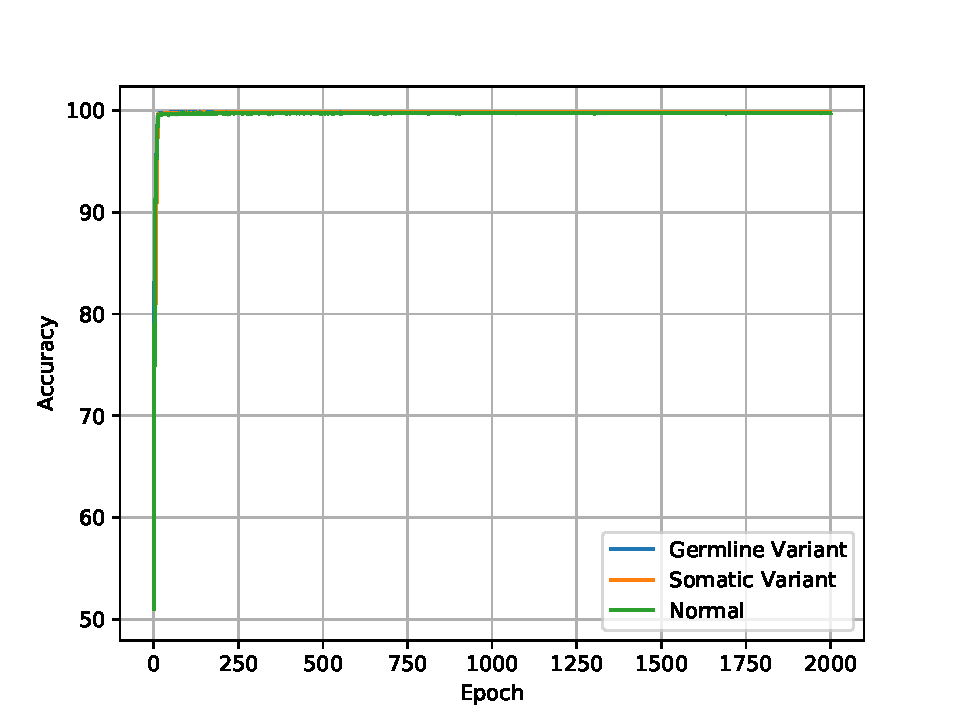
\includegraphics[width = 3in]{Transformer_Train_Accuracy}}
\subfloat[]{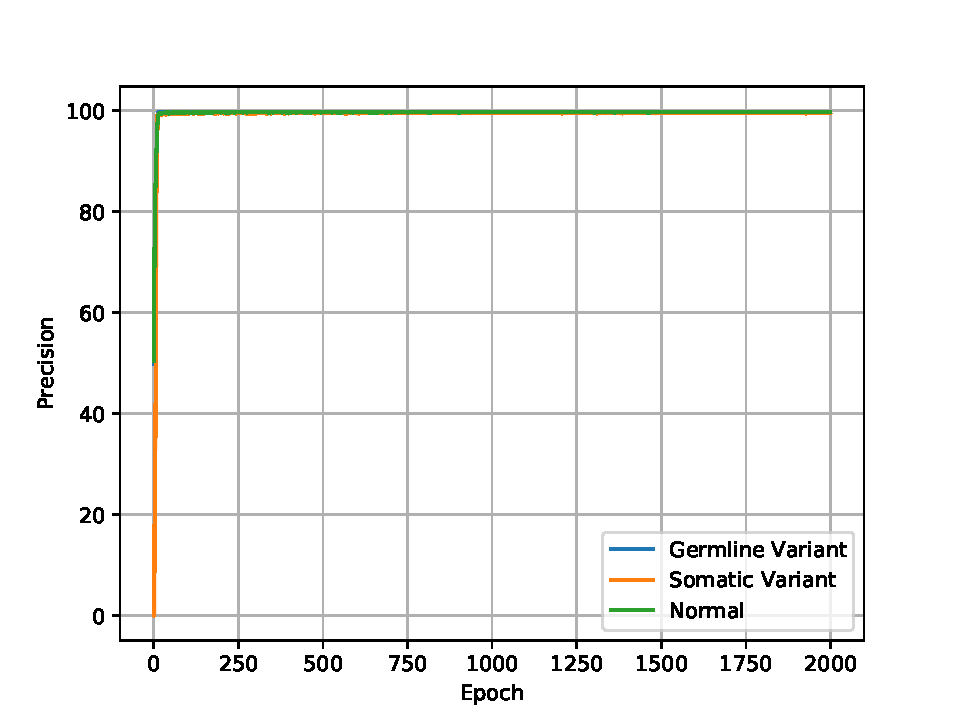
\includegraphics[width = 3in]{Transformer_Train_Precision}} \\
\subfloat[]{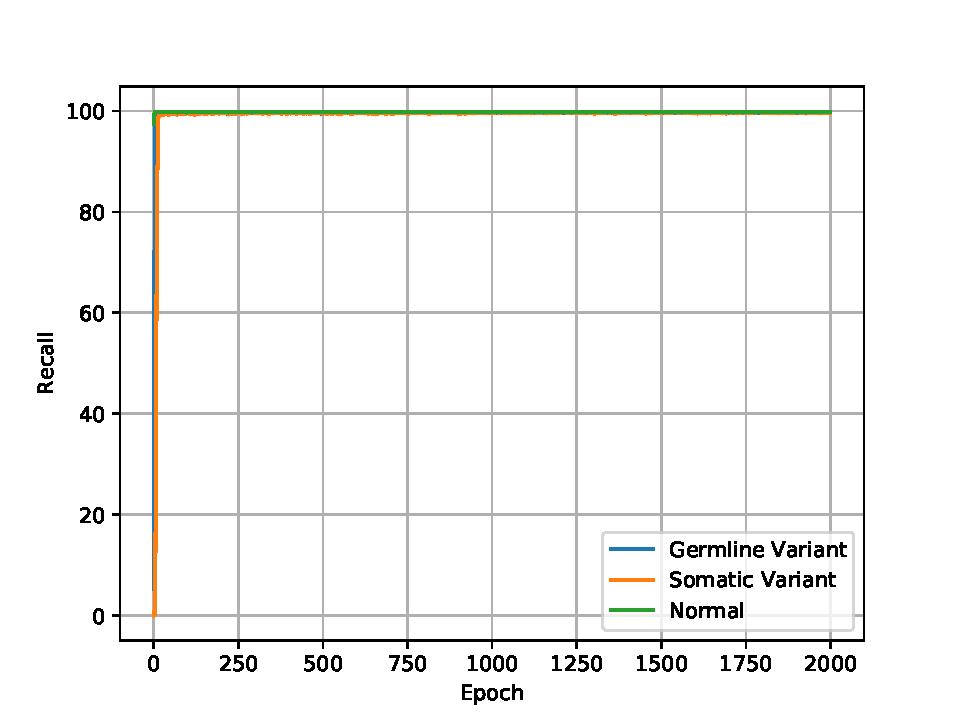
\includegraphics[width = 3in]{Transformer_Train_Recall}}
\subfloat[]{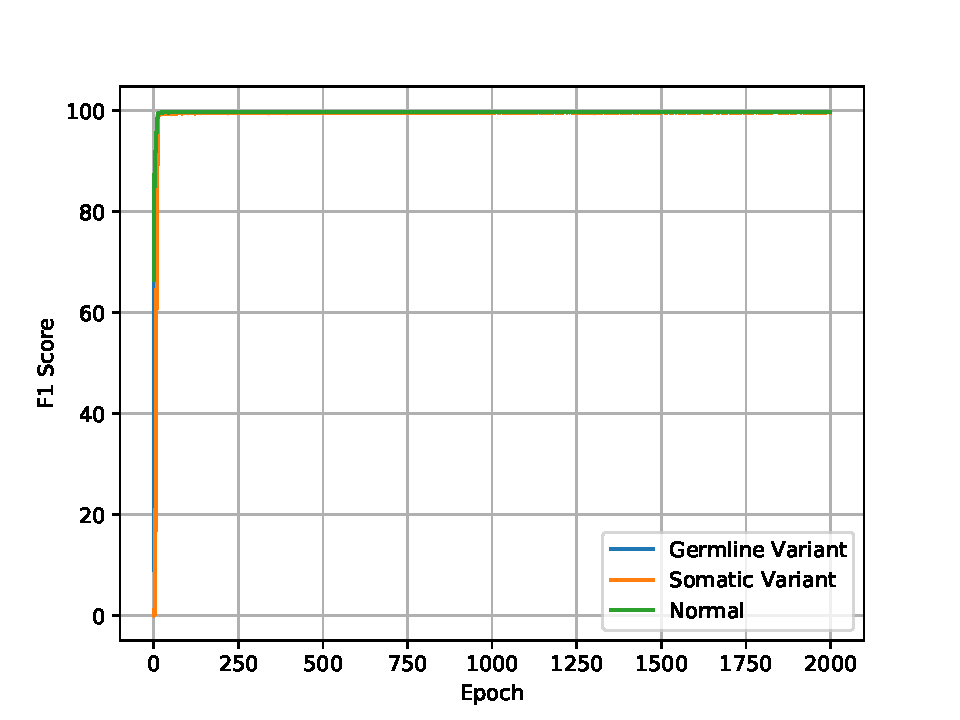
\includegraphics[width = 3in]{Transformer_Train_F1 Score}} \\
\setlength{\belowcaptionskip}{0pt}
\caption{Training set performance of the Transformer model on the modified data.}
\end{center}
\end{figure}

\begin{figure}
\begin{center}
\subfloat[]{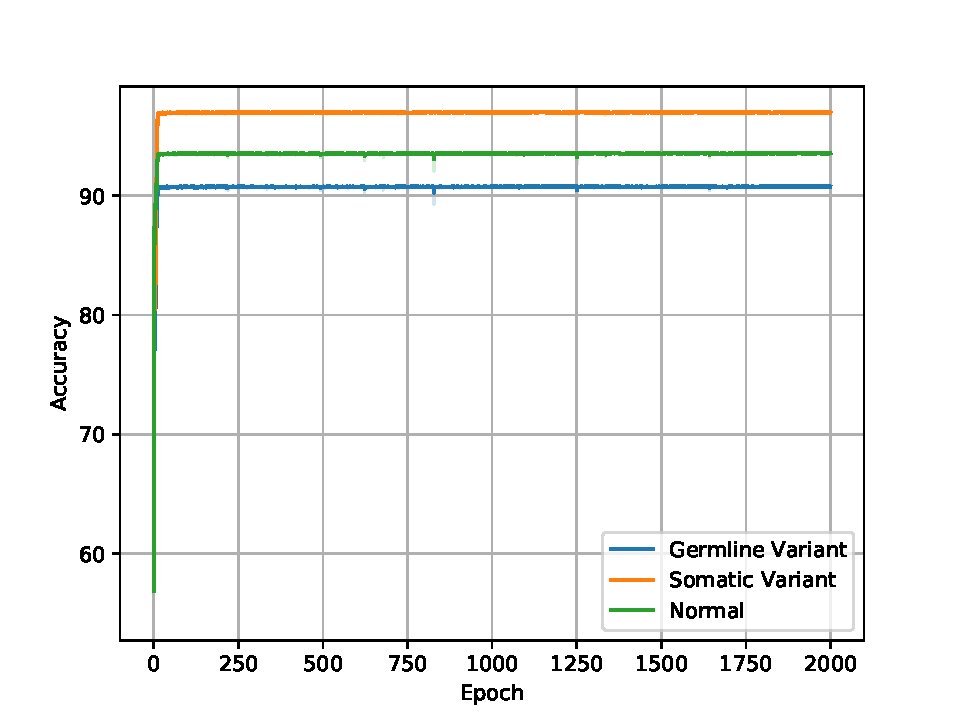
\includegraphics[width = 3in]{Transformer_Valid_Accuracy}}
\subfloat[]{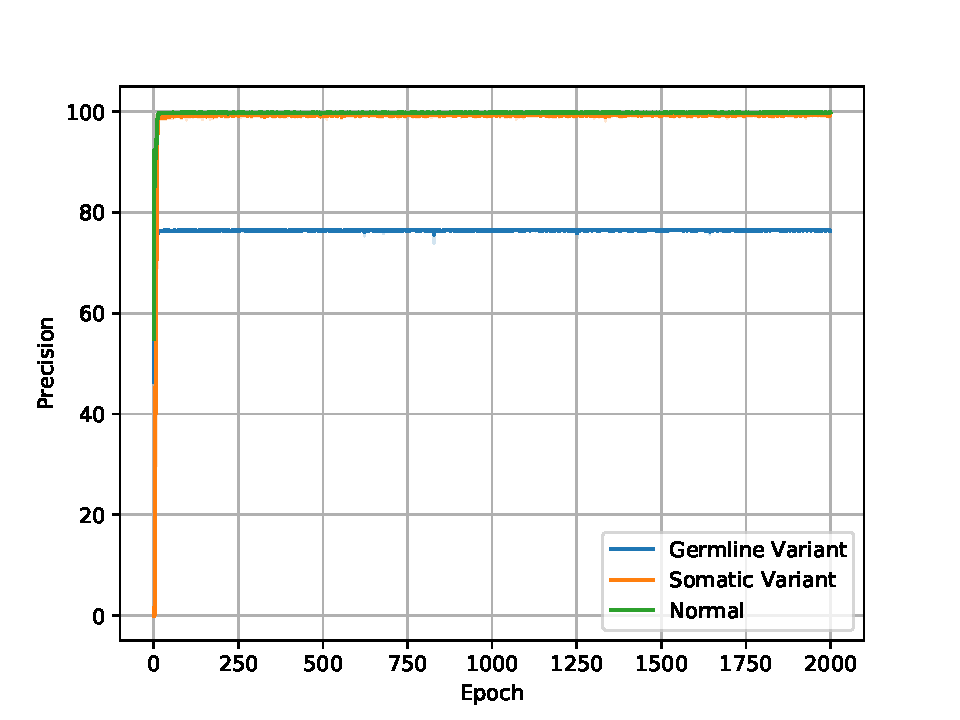
\includegraphics[width = 3in]{Transformer_Valid_Precision}} \\
\subfloat[]{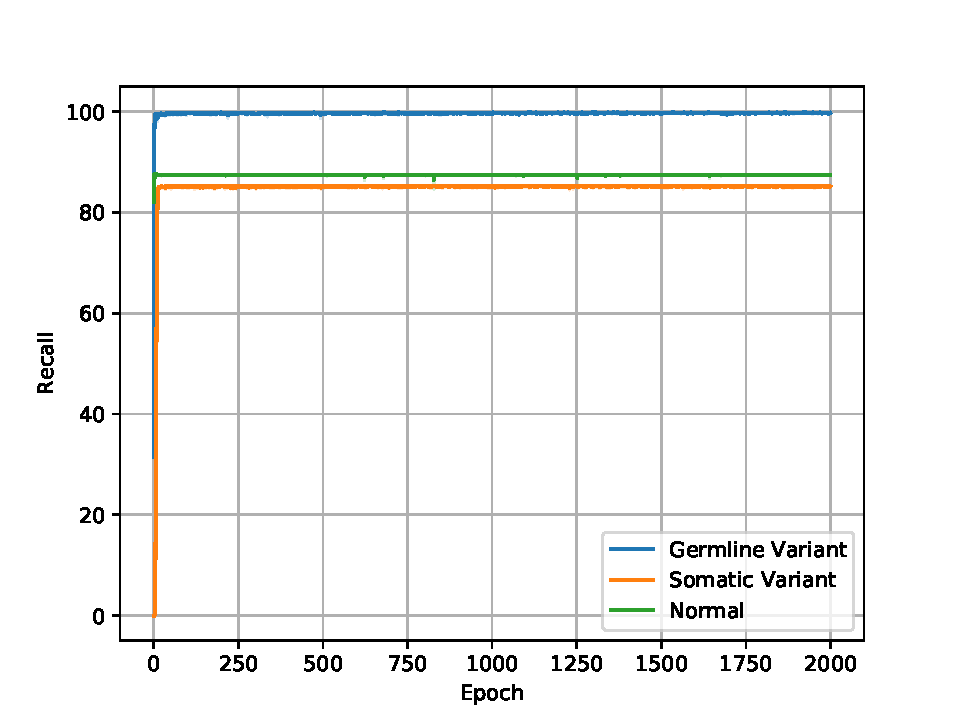
\includegraphics[width = 3in]{Transformer_Valid_Recall}}
\subfloat[]{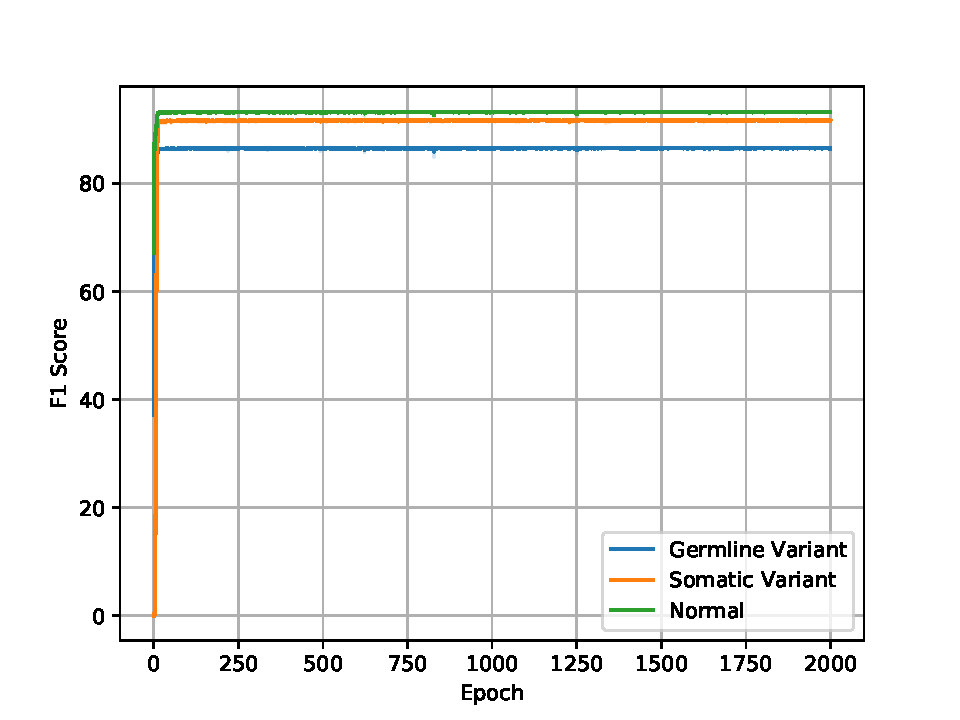
\includegraphics[width = 3in]{Transformer_Valid_F1 Score}} \\
\subfloat[]{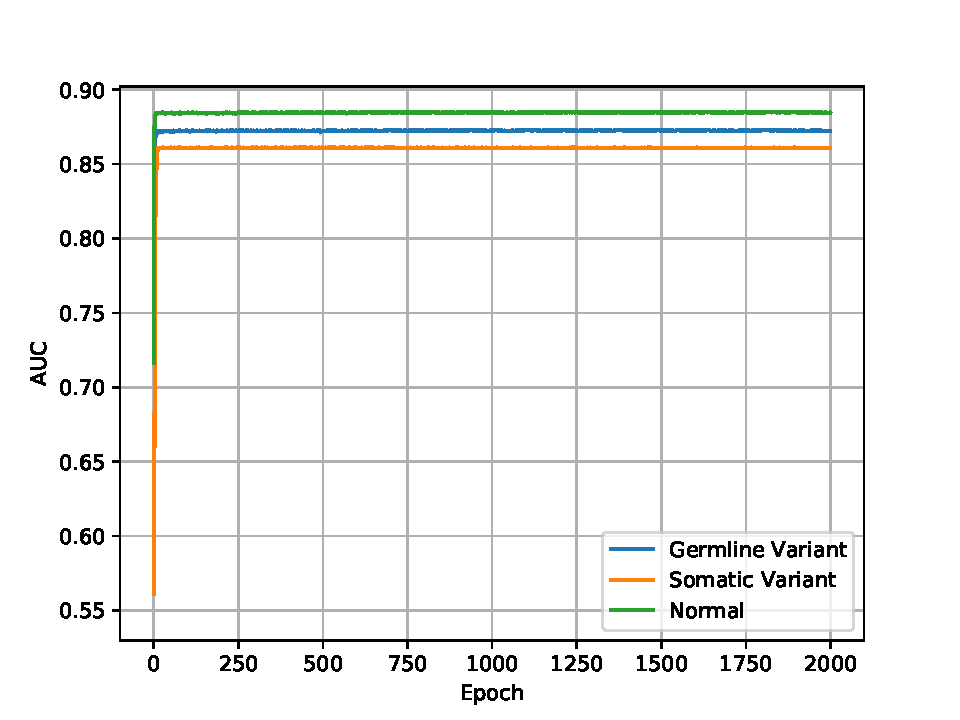
\includegraphics[width = 3in]{Transformer_Valid_AUC}}
\setlength{\belowcaptionskip}{0pt}
\caption{Validation set performance of the Transformer model on the modified data.}
\end{center}
\end{figure}

\begin{figure}
\begin{center}
\subfloat[]{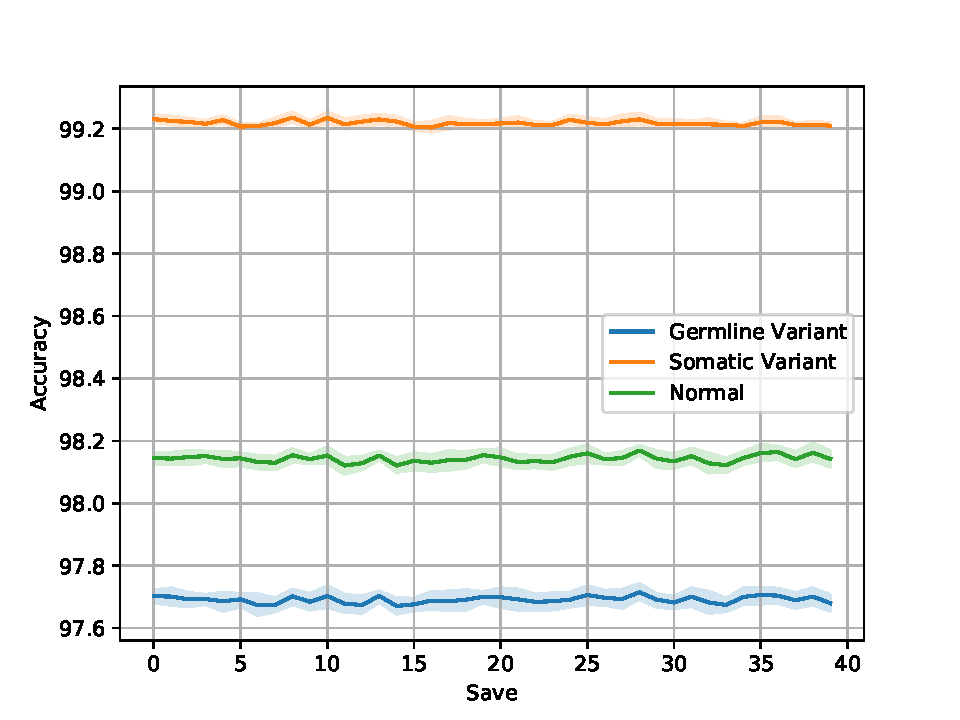
\includegraphics[width = 3in]{Transformer_Test_Accuracy}}
\subfloat[]{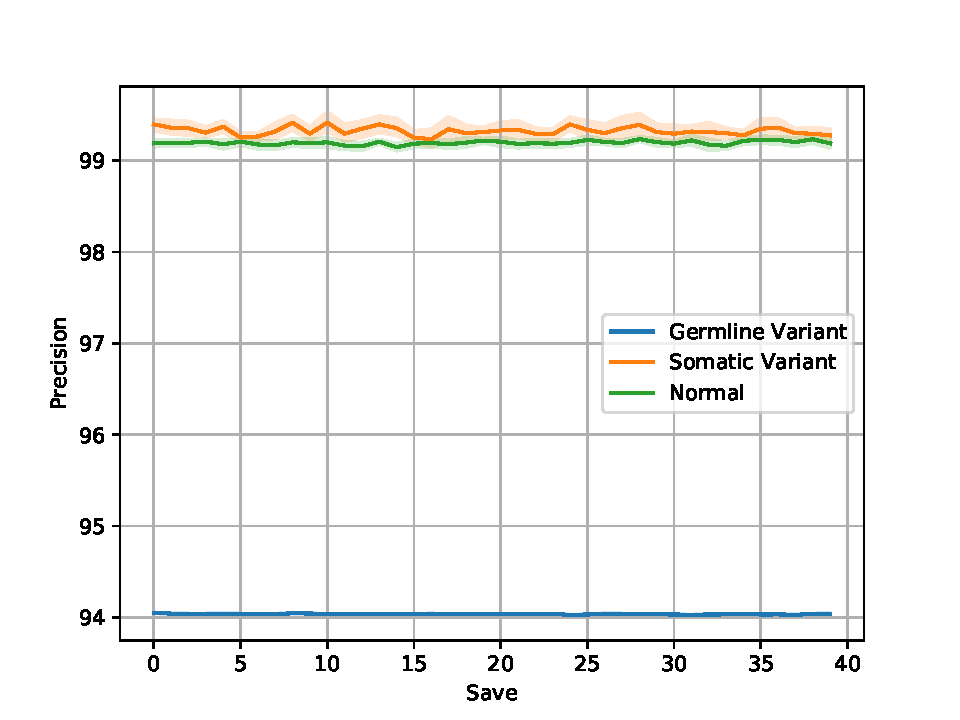
\includegraphics[width = 3in]{Transformer_Test_Precision}} \\
\subfloat[]{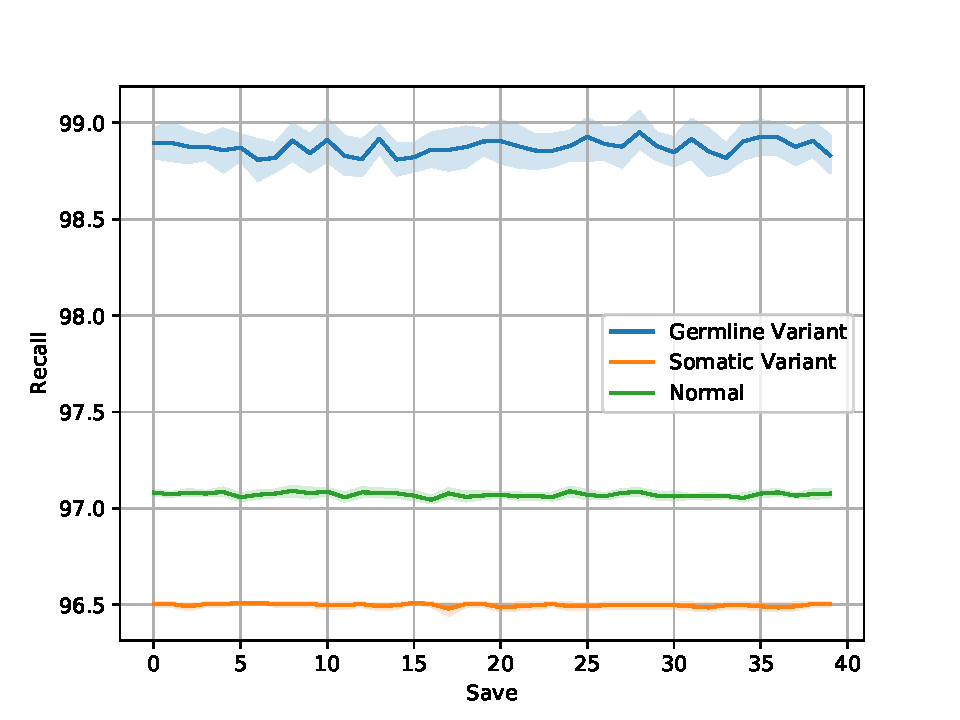
\includegraphics[width = 3in]{Transformer_Test_Recall}}
\subfloat[]{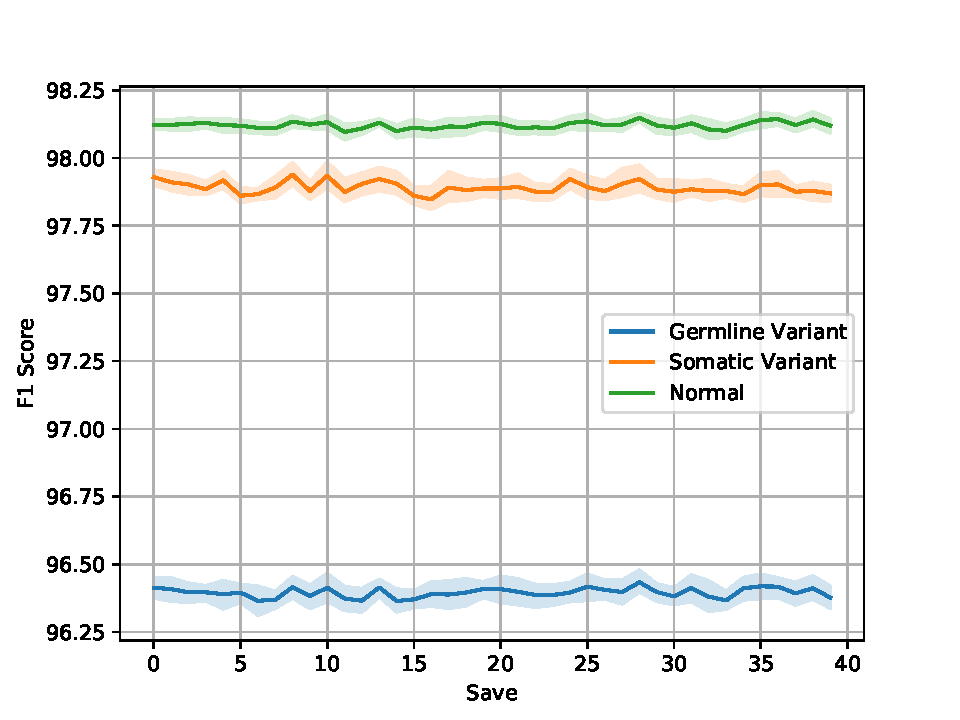
\includegraphics[width = 3in]{Transformer_Test_F1 Score}} \\
\subfloat[]{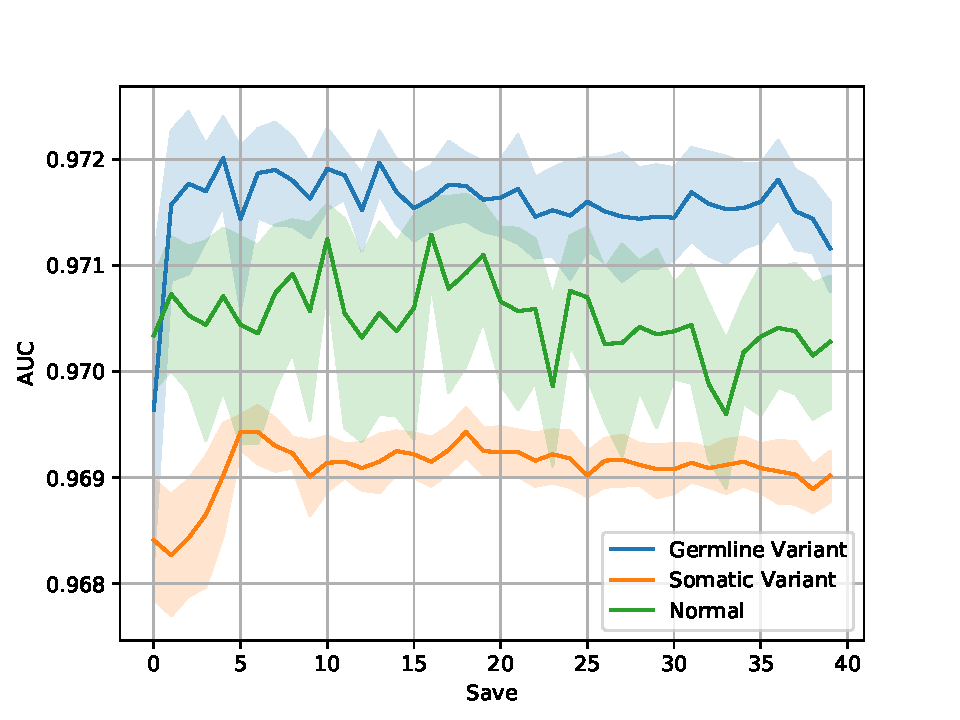
\includegraphics[width = 3in]{Transformer_Test_AUC}}
\setlength{\belowcaptionskip}{0pt}
\caption{Test set performance of the Transformer model on the modified data.}
\end{center}
\end{figure}

\begin{figure}
\begin{center}
\subfloat[]{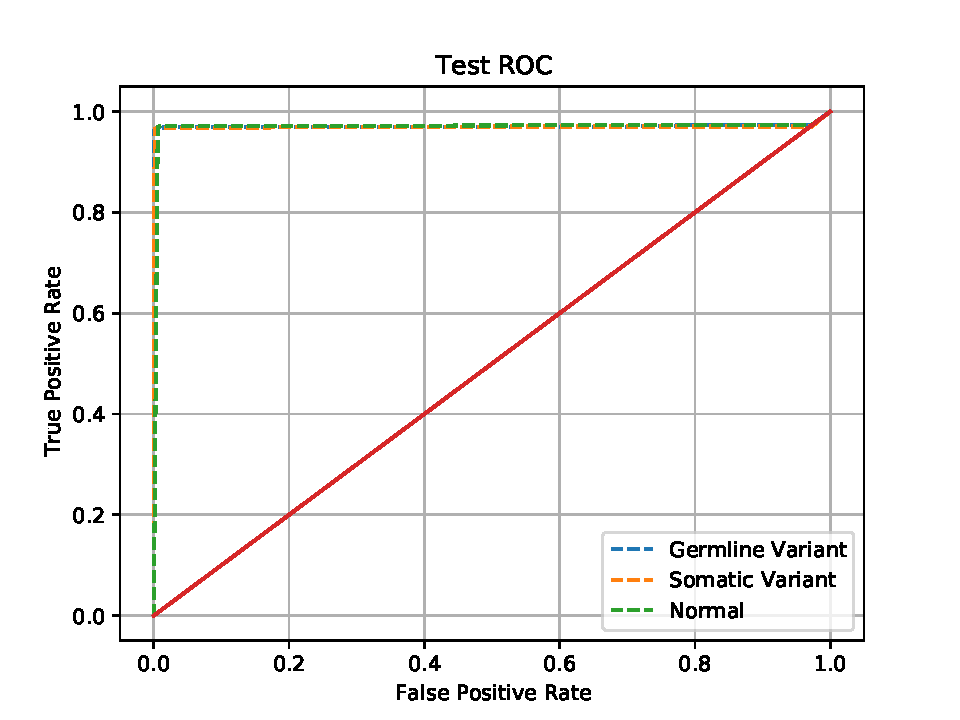
\includegraphics[width = 3in]{Transformer_Test_ROC}}
\subfloat[]{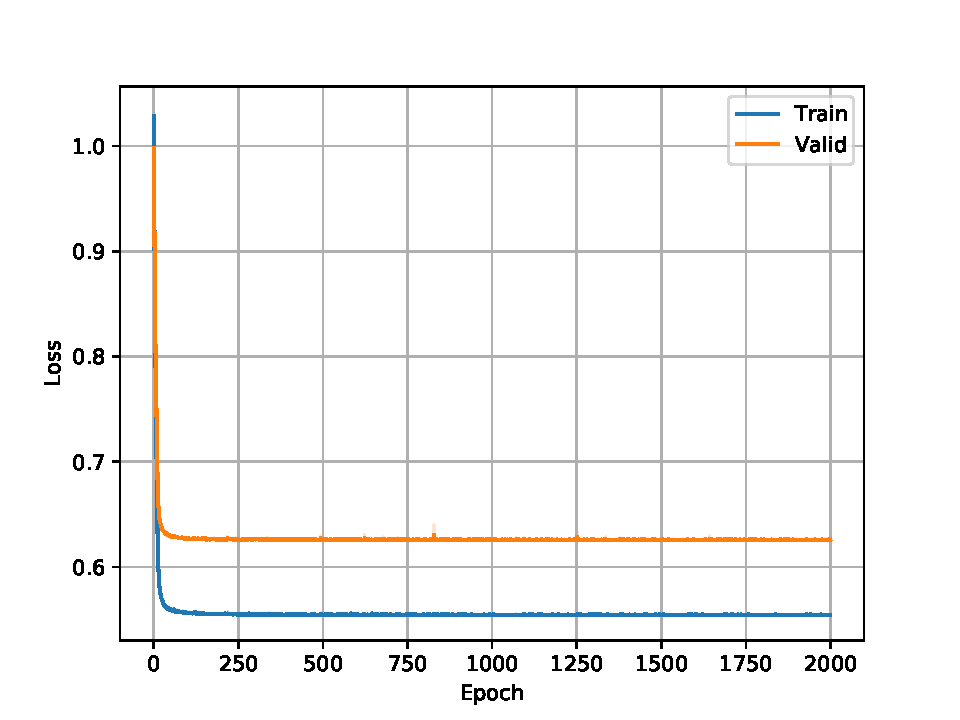
\includegraphics[width = 3in]{Transformer_Loss}}
\setlength{\belowcaptionskip}{0pt}
\caption{Test set sample ROC and loss curve for the Transformer model on the modified data}
\end{center}
\end{figure}

\section{Genotyping Task}

In the genotyping task the specific base, A, T, C or G is predicted based on the fractions of reads supporting each base and the existance of a gap in the normal and tumor samples as the the data features. Each datapoint contained 10 rows and 81 columns (same context window as for the classification task). The outputs are one-hot encoded vectors representing the bases from which it is easy to decode the actual base predicted. In this task all metrics were averaged over the four possible bases which is reflected on all figures produced as well.

\subsection{Results}

The first set of experiments for this task were run only for the models that performed best in the classification task, similarly to how it was done there when the training time was doubled. Here the models were also trained for 2000 epochs, and all on the original data.

The results are shown in a similar fashion to before on Tables 4.13-4.16. The performance is generally lower but it is apparent that the Perceptron still does the best on the training and validation sets. Surprisingly, the bidirectional GRU with 5\% dropout performs rather poorly. On the test set the Transformer beats all other models.

\begin{table}
\begin{center}
\caption{Genotyping task training set results}
\resizebox{12cm}{!}{
\begin{tabular}{ |p{6cm}||p{2.5cm}|p{2.5cm}|p{2.5cm}|p{2.5cm}| }
 \hline
 \multicolumn{5}{|c|}{Genotyping Task, Training Set Results} \\
 \hline
 \textbf{Model} & \textbf{Accuracy} & \textbf{Precision} & \textbf{Recall} &  \textbf{F1 Score}\\
 \hline
 GRU  & \small{86.44$ \%~\pm $ 0.36} & \small{73.6$ \%~\pm $ 0.65} & \small{71.27$ \%~\pm $ 0.8} & \small{72.41$ \%~\pm $ 0.72} \\ 
 \hline
 Perceptron & \textbf{\small{94.2$ \%~\pm $ 0.01}} & \textbf{\small{88.63$ \%~\pm $ 0.02}} & \textbf{\small{87.97$ \%~\pm $ 0.03}} & \textbf{\small{88.3$ \%~\pm $ 0.02}} \\
 \hline
 Bidirectional GRU + 5\% Dropout & \small{90.04$ \%~\pm $ 0.17} & \small{80.31$ \%~\pm $ 0.33} & \small{79.14$ \%~\pm $ 0.41} & \small{79.72$ \%~\pm $ 0.36} \\
 \hline
 Transformer & \small{93.85$ \%~\pm $ 0.02} & \small{87.78$ \%~\pm $ 0.04} & \small{87.38$ \%~\pm $ 0.05} & \small{87.58$ \%~\pm $ 0.04} \\
 \hline

\end{tabular}
}
\end{center}
\vskip -5mm
\end{table}

\begin{table}
\begin{center}
\caption{Genotyping task validation set results}
\resizebox{12cm}{!}{
\begin{tabular}{ |p{6cm}||p{2.5cm}|p{2.5cm}|p{2.5cm}|p{2.5cm}| }
 \hline
 \multicolumn{5}{|c|}{Genotyping Task, Validation Set Results} \\
 \hline
 \textbf{Model} & \textbf{Accuracy} & \textbf{Precision} & \textbf{Recall} &  \textbf{F1 Score}\\
 \hline
 GRU  & \small{65.1$ \%~\pm $ 0.19} & \small{29.94$ \%~\pm $ 0.4} & \small{29.6$ \%~\pm $ 0.34} & \small{29.77$ \%~\pm $ 0.37} \\ 
 \hline
 Perceptron & \textbf{\small{99.42$ \%~\pm $ 0.03}} & \textbf{\small{98.86$ \%~\pm $ 0.05}} & \textbf{\small{98.82$ \%~\pm $ 0.06}} & \textbf{\small{98.84$ \%~\pm $ 0.06}} \\
 \hline
 Bidirectional GRU + 5\% Dropout & \small{65.59$ \%~\pm $ 0.29} & \small{31.01$ \%~\pm $ 0.58} & \small{30.78$ \%~\pm $ 0.56} & \small{30.89$ \%~\pm $ 0.57} \\
 \hline
 Transformer & \small{93.46$ \%~\pm $ 0.27} & \small{89.61$ \%~\pm $ 0.54} & \small{86.88$ \%~\pm $ 0.53} & \small{88.22$ \%~\pm $ 0.53} \\
 \hline

\end{tabular}
}
\end{center}
\vskip -3mm
\end{table}

\begin{table}
\begin{center}
\caption{Genotyping task test set results}
\resizebox{12cm}{!}{
\begin{tabular}{ |p{6cm}||p{2.5cm}|p{2.5cm}|p{2.5cm}|p{2.5cm}| }
 \hline
 \multicolumn{5}{|c|}{Genotyping Task, Test Set Results} \\
 \hline
 \textbf{Model} & \textbf{Accuracy} & \textbf{Precision} & \textbf{Recall} &  \textbf{F1 Score}\\
 \hline
 GRU  & \small{64.27$ \%~\pm $ 0.09} & \small{28.38$ \%~\pm $ 0.18} & \small{28.29$ \%~\pm $ 0.18} & \small{28.33$ \%~\pm $ 0.18} \\ 
 \hline
 Perceptron & \small{88.51$ \%~\pm $ 0.03} & \small{77.42$ \%~\pm $ 0.06} & \small{76.82$ \%~\pm $ 0.06} & \small{77.12$ \%~\pm $ 0.06} \\
 \hline
 Bidirectional GRU + 5\% Dropout & \small{64.22$ \%~\pm $ 0.07} & \small{28.32$ \%~\pm $ 0.14} & \small{28.28$ \%~\pm $ 0.13} & \small{28.3$ \%~\pm $ 0.14} \\
 \hline
 Transformer & \textbf{\small{89.27$ \%~\pm $ 0.12}} & \textbf{\small{79.06$ \%~\pm $ 0.23}} & \textbf{\small{78.34$ \%~\pm $ 0.2}} & \textbf{\small{78.7$ \%~\pm $ 0.23}} \\
 \hline

\end{tabular}
}
\end{center}
\vskip -3mm
\end{table}

\begin{table}
\begin{center}
\caption{AUC metric results on the genotyping task}
\resizebox{12cm}{!}{
\begin{tabular}{ |p{6cm}||p{3cm}|p{3cm}| }
 \hline
 \multicolumn{3}{|c|}{Genotyping Task, AUCs} \\
 \hline
 \textbf{Model} & \textbf{Validation AUC} & \textbf{Test AUC} \\
 \hline
 GRU  & \small{0.5494$ ~\pm $ 0.0034} & \small{0.5346$ ~\pm $ 0.0025} \\ 
 \hline
 Perceptron & \textbf{\small{0.9998$ ~\pm $ 0.0}} & \small{0.8877$ ~\pm $ 0.0003} \\
 \hline
 Bidirectional GRU + 5\% Dropout & \small{0.5522$ ~\pm $ 0.0039} & \small{0.5315$ ~\pm $ 0.0018} \\
 \hline
 Transformer$ $ & \small{0.8735$ ~\pm $ 0.0006} & \textbf{\small{0.9074$ ~\pm $ 0.002}} \\
 \hline

\end{tabular}
}
\end{center}
\vskip -5mm
\end{table}

% Data tweak

After the data were modified all of the models were trained have results to compare to the classification task and the previous ones mentioned above. These are displayed in Tables 4.17-4.20.

Curiously, what happens on this task with the new data is somewhat opposed to what happened to the classification results. The performance of the simple recurrent models and the GRU variants increase while those of the Perceptron and Transformer decrease.

Overall, the Transformer usually dominates all metrics, even on the training and validation sets.

\begin{table}
\begin{center}
\caption{Training set results of the genotyping task on the modified data}
\resizebox{12cm}{!}{
\begin{tabular}{ |p{6cm}||p{2.5cm}|p{2.5cm}|p{2.5cm}|p{2.5cm}| }
 \hline
 \multicolumn{5}{|c|}{Modified Data, Genotyping Task, Training Set Results} \\
 \hline
 \textbf{Model} & \textbf{Accuracy} & \textbf{Precision} & \textbf{Recall} &  \textbf{F1 Score}\\
 \hline
 GRU  & \small{87.14$ \%~\pm $ 0.4} & \small{75.45$ \%~\pm $ 0.65} & \small{72.66$ \%~\pm $ 0.89} & \small{74.02$ \%~\pm $ 0.76} \\ 
 \hline
 LSTM & \small{86.99$ \%~\pm $ 1.15} & \small{74.62$ \%~\pm $ 2.26} & \small{72.44$ \%~\pm $ 2.38} & \small{73.51$ \%~\pm $ 2.32} \\
 \hline
 Vanilla RNN & \small{78.24$ \%~\pm $ 1.15} & \small{56.99$ \%~\pm $ 2.38} & \small{54.27$ \%~\pm $ 2.26} & \small{55.6$ \%~\pm $ 2.32} \\
 \hline
 Perceptron & \small{91.61$ \%~\pm $ 0.01} & \small{83.28$ \%~\pm $ 0.02} & \small{83.1$ \%~\pm $ 0.03} & \small{83.19$ \%~\pm $ 0.02} \\
 \hline
 GRU + 5\% Dropout & \small{86.35$ \%~\pm $ 0.31} & \small{73.52$ \%~\pm $ 0.57} & \small{71.0$ \%~\pm $ 0.7} & \small{72.23$ \%~\pm $ 0.62} \\
 \hline
 GRU + 10\% Dropout & \small{85.97$ \%~\pm $ 0.19} & \small{72.57$ \%~\pm $ 0.35} & \small{70.38$ \%~\pm $ 0.44} & \small{71.46$ \%~\pm $ 0.39} \\
 \hline
 Bidirectional GRU & \small{91.66$ \%~\pm $ 0.22} & \small{83.85$ \%~\pm $ 0.37} & \small{82.32$ \%~\pm $ 0.49} & \small{83.08$ \%~\pm $ 0.43} \\
 \hline
 Bidirectional GRU + 5\% Dropout & \small{91.16$ \%~\pm $ 0.12} & \small{82.8$ \%~\pm $ 0.25} & \small{81.32$ \%~\pm $ 0.27} & \small{82.06$ \%~\pm $ 0.25} \\
 \hline
 Bidirectional GRU + 10\% Dropout & \small{90.58$ \%~\pm $ 0.15} & \small{81.53$ \%~\pm $ 0.29} & \small{80.06$ \%~\pm $ 0.34} & \small{80.79$ \%~\pm $ 0.31} \\
 \hline
 Transformer & \textbf{\small{93.44$ \%~\pm $ 0.05}} & \textbf{\small{86.89$ \%~\pm $ 0.1}} & \textbf{\small{86.65$ \%~\pm $ 0.11}} & \textbf{\small{86.76$ \%~\pm $ 0.11}} \\
 \hline

\end{tabular}
}
\end{center}
\vskip -5mm
\end{table}

\begin{table}
\begin{center}
\caption{Validation set results of the genotyping task on the modified data}
\resizebox{12cm}{!}{
\begin{tabular}{ |p{6cm}||p{2.5cm}|p{2.5cm}|p{2.5cm}|p{2.5cm}| }
 \hline
 \multicolumn{5}{|c|}{Modified Data, Genotyping Task, Validation Set Results} \\
 \hline
 \textbf{Model} & \textbf{Accuracy} & \textbf{Precision} & \textbf{Recall} &  \textbf{F1 Score}\\
 \hline
 GRU  & \small{69.17$ \%~\pm $ 0.26} & \small{38.2$ \%~\pm $ 0.5} & \small{37.51$ \%~\pm $ 0.54} & \small{37.85$ \%~\pm $ 0.51} \\ 
 \hline
 LSTM & \small{69.6$ \%~\pm $ 0.24} & \small{39.32$ \%~\pm $ 0.51} & \small{38.45$ \%~\pm $ 0.51} & \small{38.88$ \%~\pm $ 0.51} \\
 \hline
 Vanilla RNN & \small{66.49$ \%~\pm $ 0.19} & \small{32.27$ \%~\pm $ 0.47} & \small{31.78$ \%~\pm $ 0.38} & \small{32.02$ \%~\pm $ 0.42} \\
 \hline
 Perceptron & \small{84.34$ \%~\pm $ 0.07} & \small{68.78$ \%~\pm $ 0.14} & \small{68.32$ \%~\pm $ 0.14} & \small{68.54$ \%~\pm $ 0.14} \\
 \hline
 GRU + 5\% Dropout & \small{69.68$ \%~\pm $ 0.19} & \small{39.13$ \%~\pm $ 0.41} & \small{38.52$ \%~\pm $ 0.41} & \small{38.82$ \%~\pm $ 0.4} \\
 \hline
 GRU + 10\% Dropout & \small{69.03$ \%~\pm $ 0.22} & \small{37.83$ \%~\pm $ 0.43} & \small{37.32$ \%~\pm $ 0.42} & \small{37.57$ \%~\pm $ 0.42} \\
 \hline
 Bidirectional GRU & \small{69.77$ \%~\pm $ 0.15} & \small{39.19$ \%~\pm $ 0.33} & \small{38.94$ \%~\pm $ 0.29} & \small{39.06$ \%~\pm $ 0.31} \\
 \hline
 Bidirectional GRU + 5\% Dropout & \small{69.4$ \%~\pm $ 0.2} & \small{38.69$ \%~\pm $ 0.44} & \small{38.27$ \%~\pm $ 0.37} & \small{38.48$ \%~\pm $ 0.4} \\
 \hline
 Bidirectional GRU + 10\% Dropout & \small{69.86$ \%~\pm $ 0.22} & \small{39.47$ \%~\pm $ 0.47} & \small{39.1$ \%~\pm $ 0.42} & \small{39.29$ \%~\pm $ 0.44} \\
 \hline
 Transformer & \textbf{\small{85.75$ \%~\pm $ 0.13}} & \textbf{\small{73.26$ \%~\pm $ 0.28}} & \textbf{\small{71.67$ \%~\pm $ 0.26}} & \textbf{\small{72.45$ \%~\pm $ 0.27}} \\
 \hline

\end{tabular}
}
\end{center}
\vskip -5mm
\end{table}

\begin{table}
\begin{center}
\caption{Test set results of the genotyping task on the modified data}
\resizebox{12cm}{!}{
\begin{tabular}{ |p{6cm}||p{2.5cm}|p{2.5cm}|p{2.5cm}|p{2.5cm}| }
 \hline
 \multicolumn{5}{|c|}{Modified Data, Genotyping Task, Test Set Results} \\
 \hline
 \textbf{Model} & \textbf{Accuracy} & \textbf{Precision} & \textbf{Recall} &  \textbf{F1 Score}\\
 \hline
 GRU  & \small{63.48$ \%~\pm $ 0.09} & \small{26.82$ \%~\pm $ 0.2} & \small{26.79$ \%~\pm $ 0.18} & \small{26.8$ \%~\pm $ 0.19} \\ 
 \hline
 LSTM & \small{63.55$ \%~\pm $ 0.09} & \small{27.02$ \%~\pm $ 0.17} & \small{26.89$ \%~\pm $ 0.17} & \small{26.95$ \%~\pm $ 0.16} \\
 \hline
 Vanilla RNN & \small{62.71$ \%~\pm $ 0.07} & \small{25.1$ \%~\pm $ 0.14} & \small{25.01$ \%~\pm $ 0.14} & \small{25.06$ \%~\pm $ 0.14}\\
 \hline
 Perceptron & \small{78.41$ \%~\pm $ 0.03} & \small{57.11$ \%~\pm $ 0.06} & \small{56.8$ \%~\pm $ 0.06} & \small{56.95$ \%~\pm $ 0.06} \\
 \hline
 GRU + 5\% Dropout & \small{63.75$ \%~\pm $ 0.08} & \small{27.34$ \%~\pm $ 0.17} & \small{27.3$ \%~\pm $ 0.16} & \small{27.32$ \%~\pm $ 0.17} \\
 \hline
 GRU + 10\% Dropout & \small{63.9$ \%~\pm $ 0.06} & \small{27.68$ \%~\pm $ 0.13} & \small{27.63$ \%~\pm $ 0.12} & \small{27.65$ \%~\pm $ 0.12} \\
 \hline
 Bidirectional GRU & \small{63.35$ \%~\pm $ 0.1} & \small{26.57$ \%~\pm $ 0.21} & \small{26.54$ \%~\pm $ 0.21} & \small{26.56$ \%~\pm $ 0.21} \\
 \hline
 Bidirectional GRU + 5\% Dropout & \small{63.43$ \%~\pm $ 0.07} & \small{26.75$ \%~\pm $ 0.13} & \small{26.7$ \%~\pm $ 0.14} & \small{26.72$ \%~\pm $ 0.13} \\
 \hline
 Bidirectional GRU + 10\% Dropout & \small{63.45$ \%~\pm $ 0.08} & \small{26.79$ \%~\pm $ 0.17} & \small{26.76$ \%~\pm $ 0.18} & \small{26.77$ \%~\pm $ 0.18} \\
 \hline
 Transformer & \textbf{\small{85.47$ \%~\pm $ 0.06}} & \textbf{\small{71.1$ \%~\pm $ 0.13}} & \textbf{\small{70.87$ \%~\pm $ 0.12}} & \textbf{\small{70.99$ \%~\pm $ 0.12}} \\
 \hline

\end{tabular}
}
\end{center}
\vskip -5mm
\end{table}

\begin{table}
\begin{center}
\caption{AUC metric results of the genotyping task on the modified data}
\resizebox{12cm}{!}{
\begin{tabular}{ |p{6cm}||p{3cm}|p{3cm}| }
 \hline
 \multicolumn{3}{|c|}{Modified Data, Genotyping Task, AUCs} \\
 \hline
 \textbf{Model} & \textbf{Validation AUC} & \textbf{Test AUC} \\
 \hline
 GRU  & \small{0.5992$ ~\pm $ 0.0036} &  \small{0.5182$ ~\pm $ 0.0016} \\ 
 \hline
 LSTM & \small{0.6073$ ~\pm $ 0.0031} & \small{0.5185$ ~\pm $ 0.0015} \\
 \hline
 Vanilla RNN & \small{0.5554$ ~\pm $ 0.0044} & \small{0.5009$ ~\pm $ 0.0015} \\
 \hline
 Perceptron & \textbf{\small{0.8366$ ~\pm $ 0.0004}} & \small{0.7677$ ~\pm $ 0.0002} \\
 \hline
 GRU + 5\% Dropout & \small{0.6104$ ~\pm $ 0.0029} & \small{0.5215$ ~\pm $ 0.0018} \\
 \hline
 GRU + 10\% Dropout & \small{0.6076$ ~\pm $ 0.0034} & \small{0.5242$ ~\pm $ 0.0011} \\
 \hline
 Bidirectional GRU & \small{0.6108$ ~\pm $ 0.003} & \small{0.5141$ ~\pm $ 0.002} \\
 \hline
 Bidirectional GRU + 5\% Dropout & \small{0.6159$ ~\pm $ 0.0034} & \small{0.5141$ ~\pm $ 0.0012} \\
 \hline
 Bidirectional GRU + 10\% Dropout & \small{0.621$ ~\pm $ 0.0043} & \small{0.5138$ ~\pm $ 0.0011} \\
 \hline
 Transformer & \small{0.817$ ~\pm $ 0.0005} & \textbf{\small{0.8614$ ~\pm $ 0.0004}} \\
 \hline

\end{tabular}
}
\end{center}
\vskip -5mm
\end{table}

\subsection{Discussion}

Running times were recorded for this task as well. Everything was run locally on the same machine with the same GPU. The time taken to train 1000 epochs before and after the modification of the data measured in hours and minutes were:

\begin{itemize}

\item GRU (and other recurrent models: 0:20 $ \rightarrow $ 0:12
\item Bidirectional GRU: 0:50 $ \rightarrow $ 0:32
\item Perceptron : 0:06 $ \rightarrow $ 0:06
\item Transformer (1 encoder layer): 3:30 $ \rightarrow $ 2:05

\end{itemize}

These are roughly similar to those of the classification task models, with the exception of the Transformer which took 1hr and 30mins longer to train before and after the change in data.

The performance of all of the models were worse than for the other task. This is expected as genotyping is harder, and there are also more classes to choose from. Still, the recurrent networks did rather poorly.

On the first set of results the Perceptron was still the best for both training and validation sets, again raising the question whether some simple linear regression would be enough for this task as well. With the new data things look much more in favour of the Transformer which this time is quite significantly ahead of the competition and is much more consistent between the validation and test sets.

A possible explanation for this last point is that the distribution of classes of more equal for this task (even though the locations considered as still germline variant, somatic variant and unmutated positions), since nucleotides are being predicted. The validation set is naively chosen as the last 10\% of the training set data, this could be improved by sampling classes from the data based on their frequency instead so the validation set's class distribution represents that of the whole data.

\begin{figure}
\begin{center}
\subfloat[]{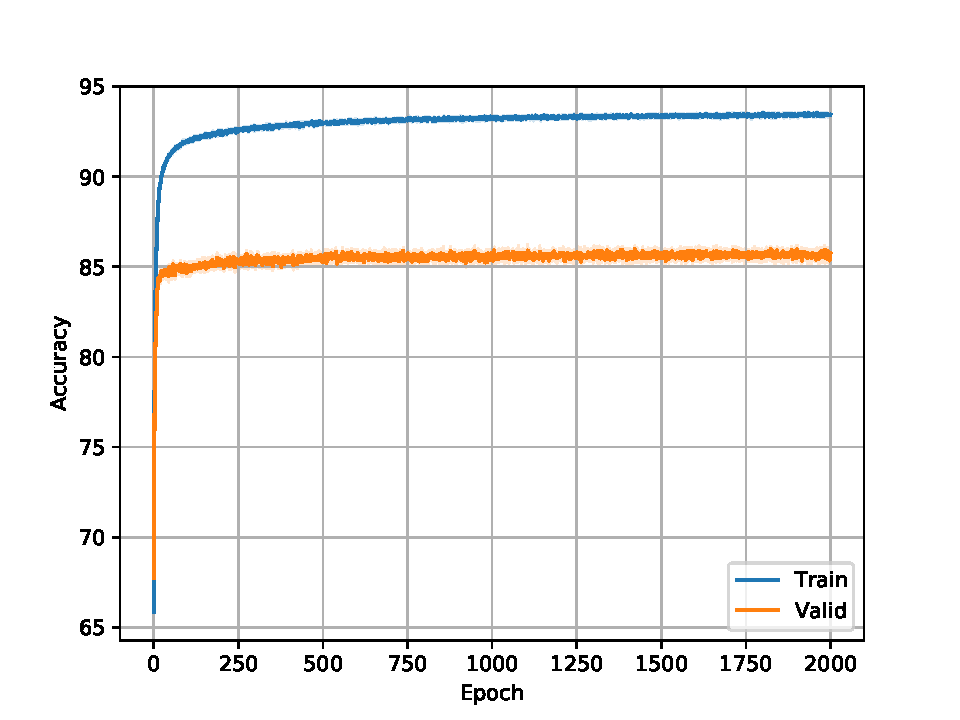
\includegraphics[width = 3in]{Genotyping_Transformer_Accuracy}}
\subfloat[]{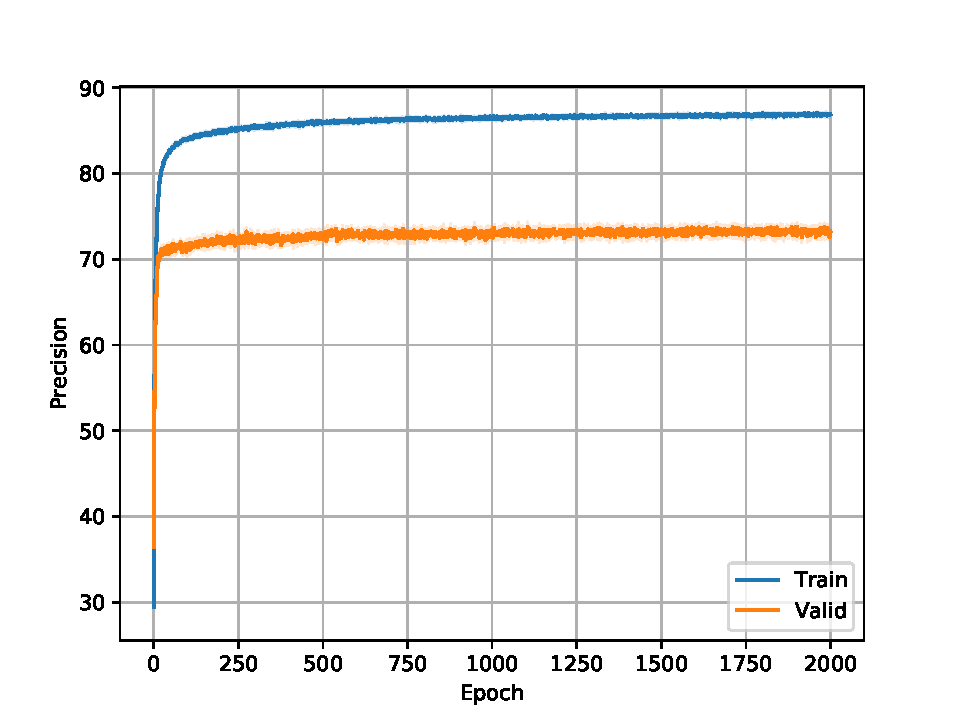
\includegraphics[width = 3in]{Genotyping_Transformer_Precision}} \\
\subfloat[]{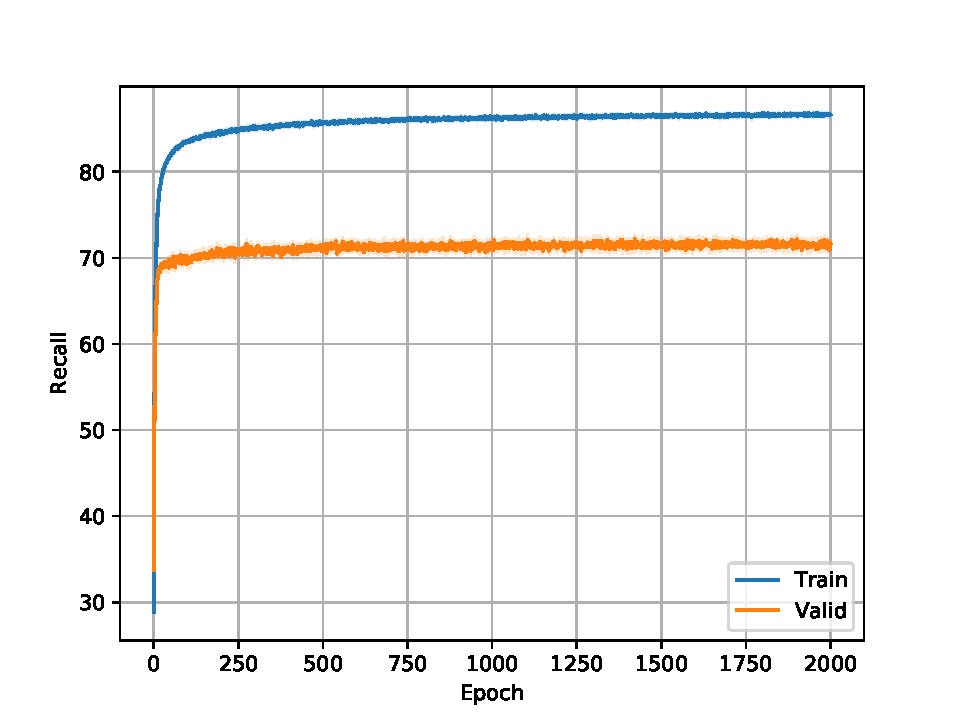
\includegraphics[width = 3in]{Genotyping_Transformer_Recall}}
\subfloat[]{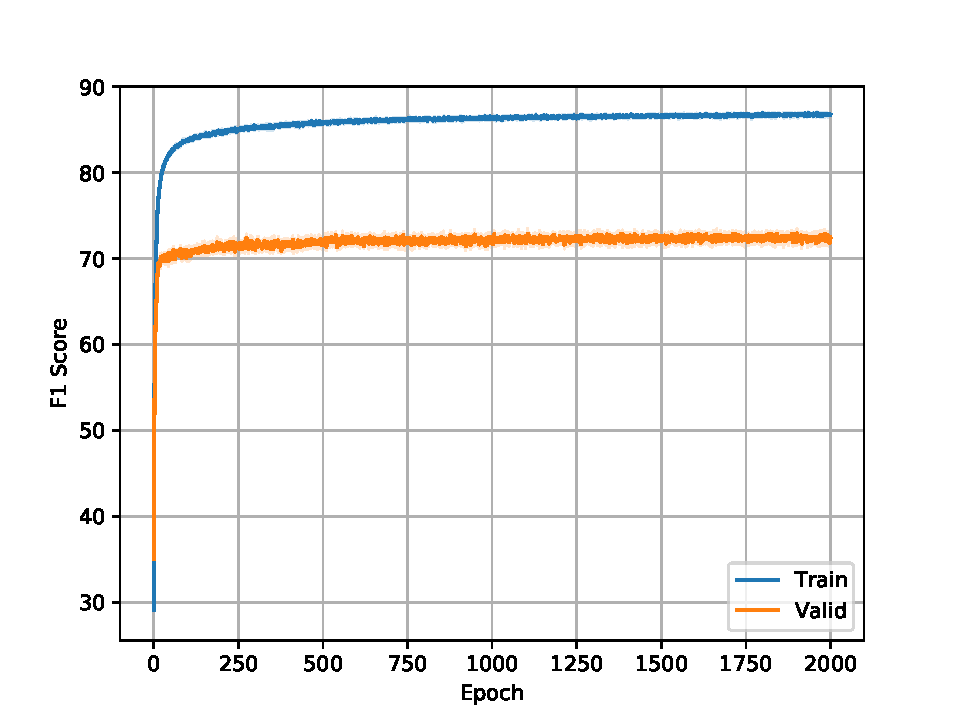
\includegraphics[width = 3in]{Genotyping_Transformer_F1 Score}} \\
\setlength{\belowcaptionskip}{0pt}
\caption{Genotyping task, training and validation set performance of the Transformer model on the modified data.}
\end{center}
\end{figure}

\begin{figure}
\begin{center}
\subfloat[]{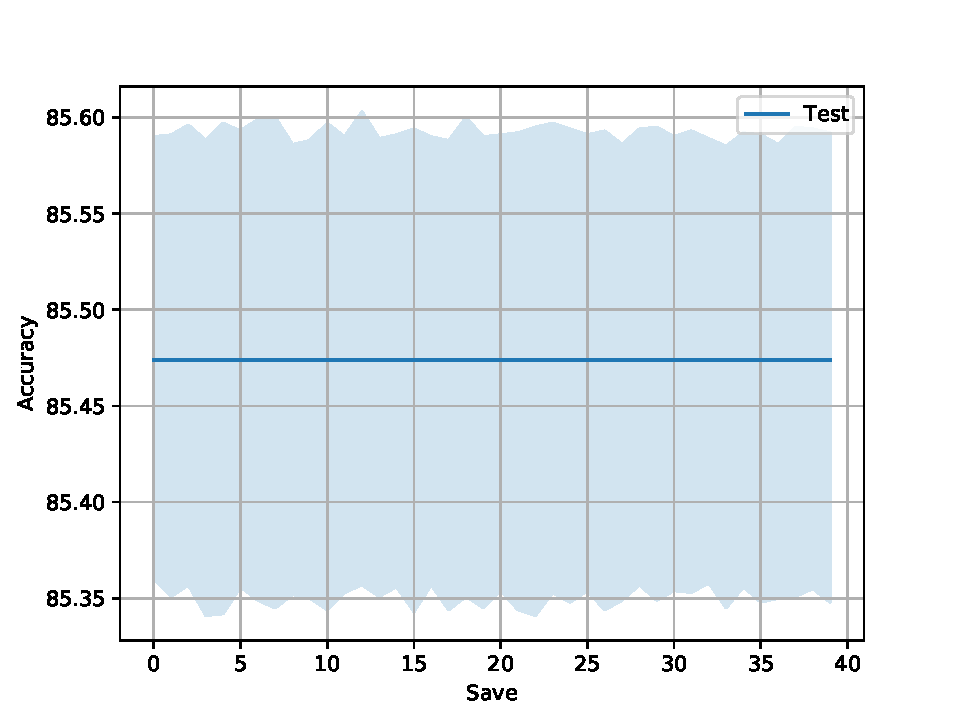
\includegraphics[width = 3in]{Genotyping_Transformer_Test_Accuracy}}
\subfloat[]{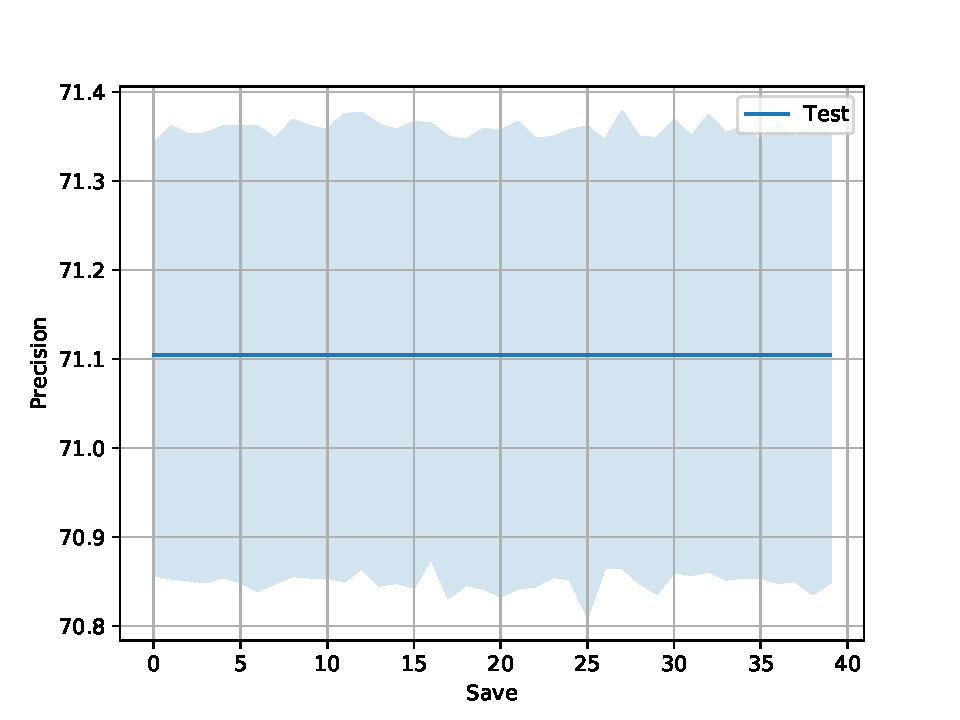
\includegraphics[width = 3in]{Genotyping_Transformer_Test_Precision}} \\
\subfloat[]{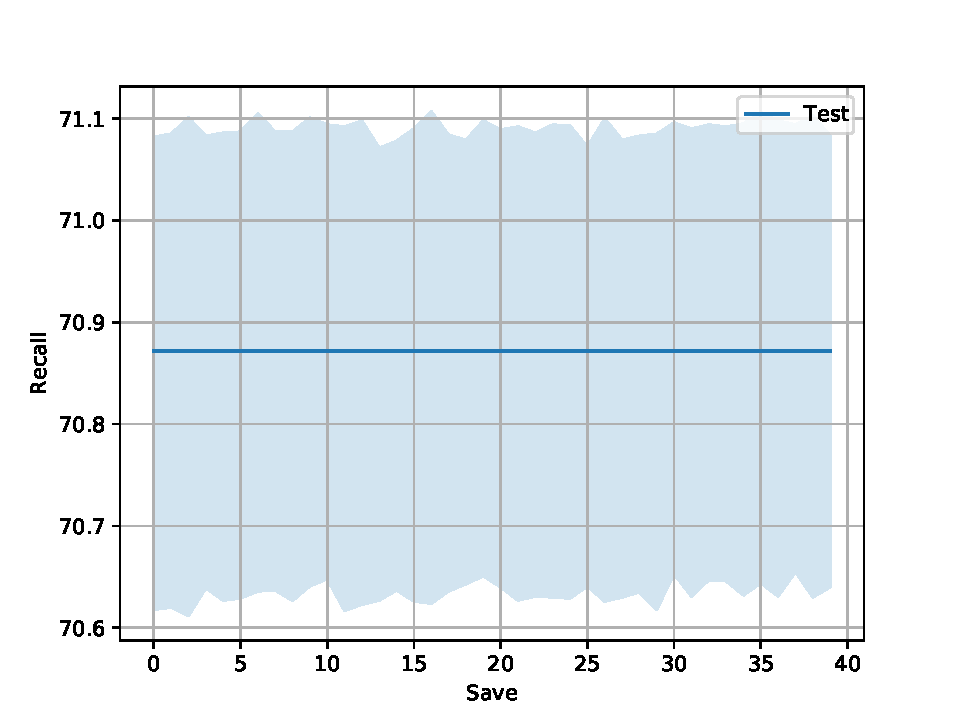
\includegraphics[width = 3in]{Genotyping_Transformer_Test_Recall}}
\subfloat[]{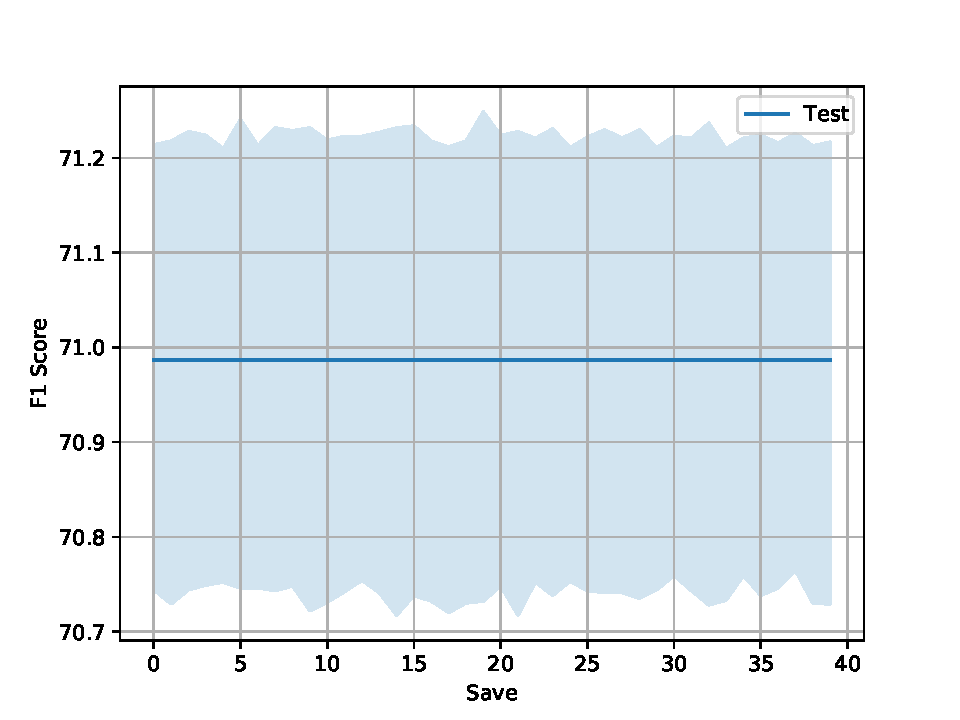
\includegraphics[width = 3in]{Genotyping_Transformer_Test_F1 Score}} \\
\subfloat[]{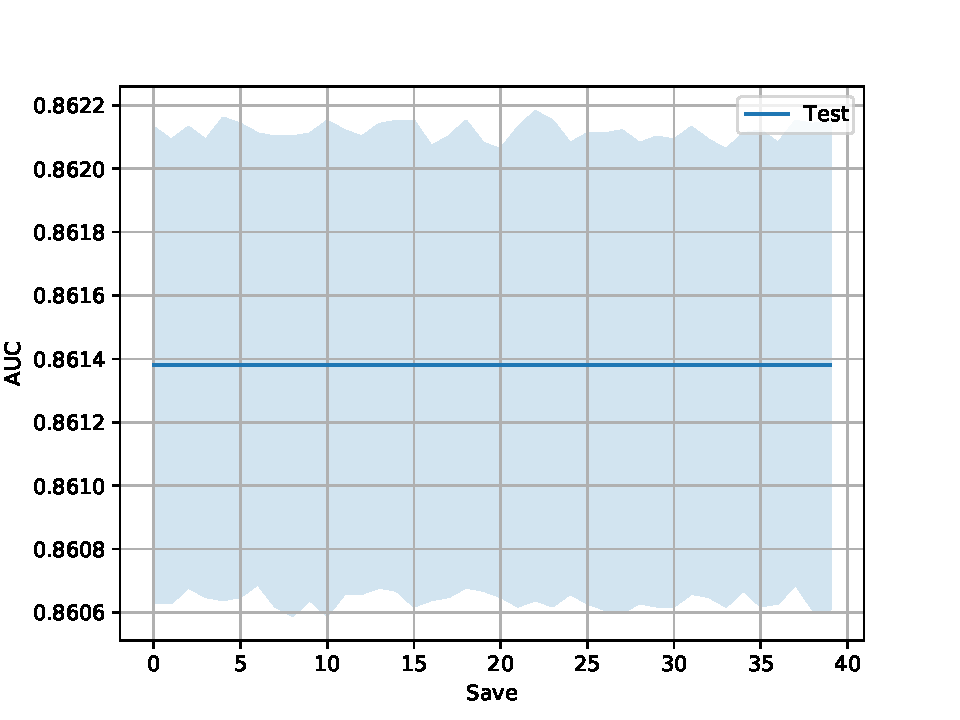
\includegraphics[width = 3in]{Genotyping_Transformer_Test_AUC}}
\setlength{\belowcaptionskip}{0pt}
\caption{Genotyping task, test set performance of the Transformer model on the modified data.}
\end{center}
\end{figure}

\begin{figure}
\begin{center}
\subfloat[]{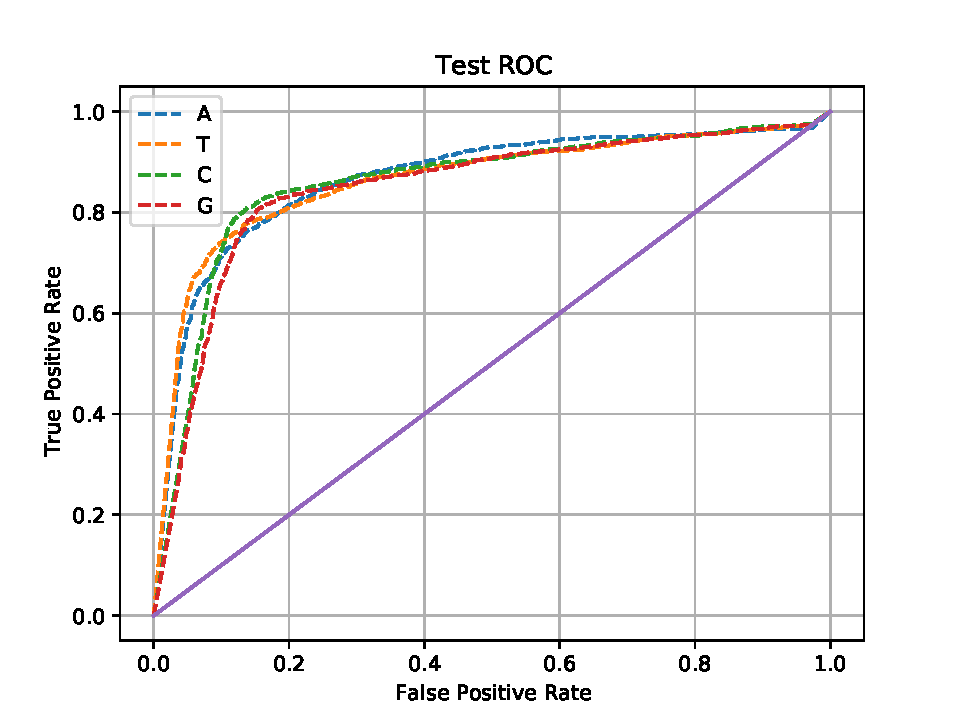
\includegraphics[width = 3in]{Genotyping_Transformer_Test_ROC}}
\subfloat[]{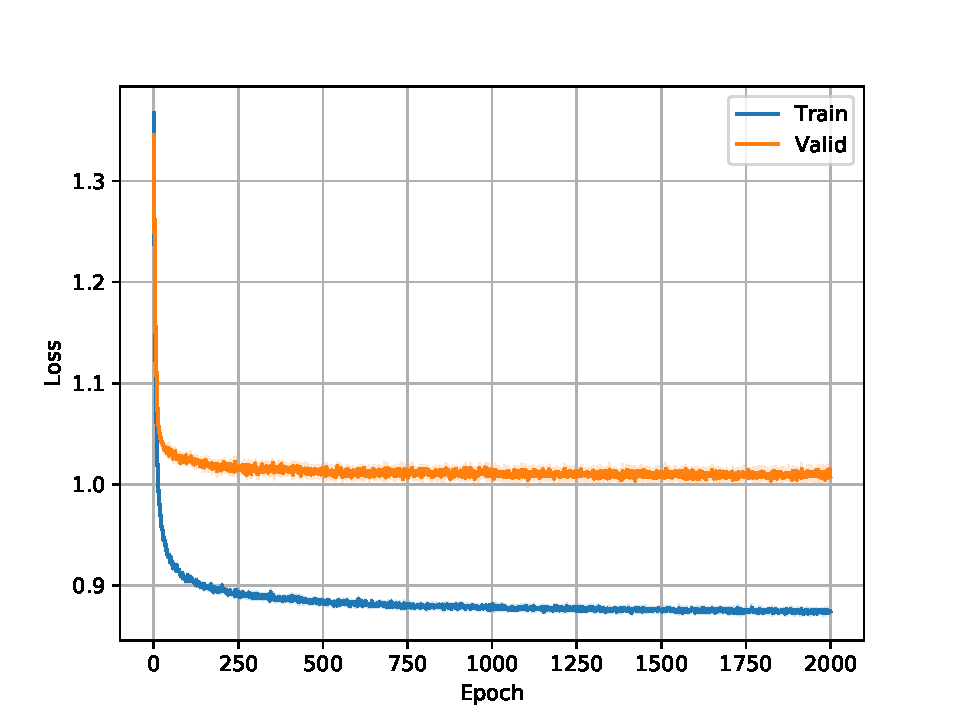
\includegraphics[width = 3in]{Genotyping_Transformer_Loss}}
\setlength{\belowcaptionskip}{0pt}
\caption{Test set sample ROC and loss curve for the Transformer model on the genotyping task with modified data}
\end{center}
\end{figure}

Figures 4.5-4.6 show example plots of the performance of the genotyping Transformer over time for the modified data. Figure 4.7 shows a sample test set run ROC curve and the evolution of the loss during the course of the training.

\section{Conclusion}

In the benchmarking study presented in chapter 1 \cite{benchmark} that inspired this project and the data used, the best F1 Score achieved by NeuSomatic \cite{neusomatic} at 60\% sample purity was around 99.21\% F1 Score. 

The closest comparison I could make in my results would be the test set performance of the Transformer model on the modified data at around 97.65\%. These results are of course hardly comparable, for a real comparison the same data would have to be used, but it shows that there is still room for improvement.

Nevertheless, NeuSomatic uses much more features and has a more complicated architecture than my models, making these results quite powerful compared to their simplicity. The experiments showcase that using Deep Learning in this type of task is worthwhile.

Using more data from different samples (from different populations) and different chromosomes to train the models could further improve results. Other architecture types could be tried as well. 

The next step would be evaluating my models on the same data NeuSomatic was tested on, and possibly evaluate NeuSomatic on my data. Due to the size of the required datasets (4TB per dataset) and the necessary processing required this did not fit into the timeline of this current project and has to left as future work.

The achieved results are encouraging and show the viability of the Transformer architecture for both the classification and genotyping tasks of somatic variant calling. The best recurrent network, which is simpler and less compute and memory intensive, can still be a good alternative that generalises better than a baseline Perceptron. Ensembling the models for the tasks could yield a useful variant caller.


\bibliographystyle{unsrt}
\bibliography{mybibfile}

%% You can include appendices like this:
% \appendix
%
% \chapter{First appendix}
%
% \section{First section}
%
% Markers do not have to consider appendices. Make sure that your contributions
% are made clear in the main body of the dissertation (within the page limit).

\end{document}
